\documentclass[main.tex]{subfiles}
\begin{document}


\chapter{NEMO detectors}\label{chap:NEMO}


%\begin{flushright}
%\textit{On peut braver les lois humaines, \\
%mais non résister aux lois naturelles}\\
%Jules Verne, \textit{Vingt mille lieues sous les mers.}
%\end{flushright} 


\NI Initiated in the late 1980s, the principal goals of the NEMO project are the search for 0$\nu\beta\beta$ and the measurement of 2$\nu\beta\beta$ decays. The strategy adopted by the collaboration is the direct detection of the two emitted electrons, by separating the $\beta\beta$ emitters from the rest of the detector. This technique also allows to investigate many $\beta\beta$ isotopes with a powerful background discrimination. The Modane Underground Laboratory (LSM), which hosted all the NEMO prototypes and detectors, is described in Section~\ref{sec:LSM}. The NEMO-3 detector is presented in Section~\ref{sec:NEMO3}. The data taken by this detector will be analyse in Chapter~6 to perform the search for the $\beta\beta$ decays of $^{\text{116}}$Cd via the excited states of $^{\text{116}}$Sn. Finally, the SuperNEMO detector is introduced in Section~\ref{sec:SuperNEMO}.


\section{Modane underground laboratory}\label{sec:LSM}


\NI Inaugurated in 1982, the Modane Underground Laboratory (LSM) \footnote{LSM : Laboratoire Souterrain de Modane in french} is located in the Frejus tunnel at the border between France and Italy as shown in Figure~\ref{LSMtunnel}.


\begin{figure}[h!]
\begin{center}
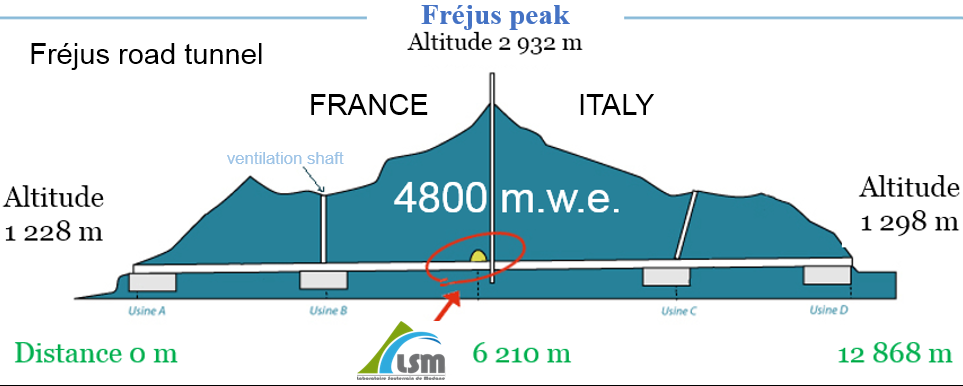
\includegraphics[scale=0.35]{pictures/Chap3/LSMtunnel.png}
\caption{Schematic view of the Modane underground laboratory location in the Frejus tunnel.}
\label{LSMtunnel}
\end{center}
\end{figure}



\NI The laboratory is sheltered from cosmic rays under 1700~m of rocks (4200 m.w.e)~\footnote{m.w.e : meter water equivalent} which makes it the deepest underground laboratory in Europe and the third one in the world. The cosmic ray flux inside the laboratory has been measured to be 4~muons/m$^\text{2}$/day~\cite{CosmicFluxLSM}, which is a reduction by a factor of one million from that at sea level. The total muon flux for different underground laboratories is presented in~Figure~\ref{LabDeepth}.
 

\begin{figure}[h!]
\begin{center}
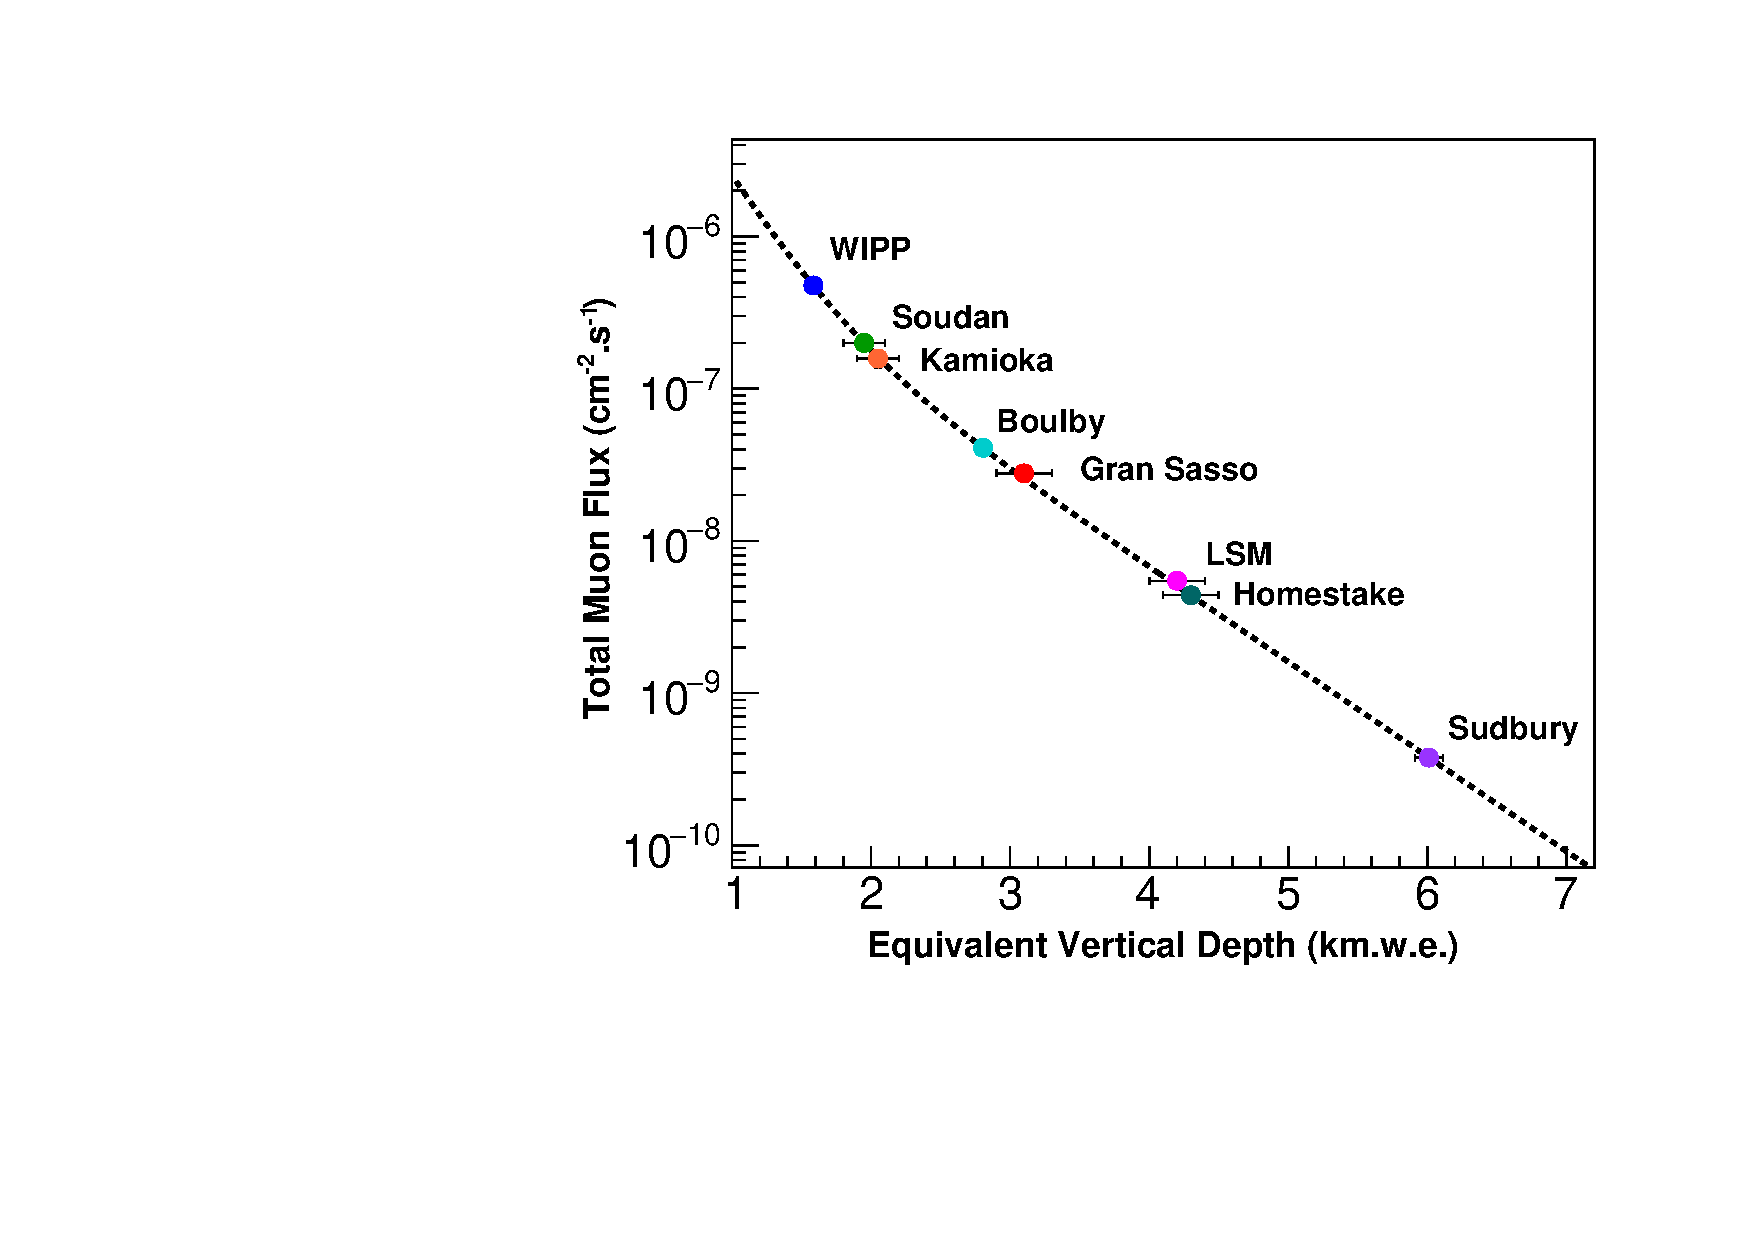
\includegraphics[scale=0.60]{pictures/Chap3/MuonFluxDifferentLab.pdf}
\caption{Total muon flux measured for various underground sites as a function of the equivalent vertical depth~\cite{MuonFluxUndergroundLab}. }
\label{LabDeepth}
\end{center}
\end{figure}


\NI The protected environment of the laboratory is very favorable to the searches of rare processes which require very low backgrounds. Initially, the laboratory hosted an experiment searching for the proton decay. Later, the laboratory diversified its activities, including astrophysics, biology, geology, electronics and environmental researches. The laboratory also has several High Purity Germanium detectors (HPGe) to measure very low radioactivity. 


\bigskip


\NI The first prototypes, NEMO-1~\cite{NEMO1} and NEMO-2~\cite{NEMO2} were installed at LSM in the late 1980s and early 1990s. Then the laboratory hosted NEMO-3 in early 2000. Today NEMO-3 has been replaced by SuperNEMO demonstrator which is currently under construction and commissionning phase.


\FloatBarrier


\section{NEMO-3}\label{sec:NEMO3}


\NI The NEMO-3 detector ran from February 2003 to January 2011 and searched for $\beta\beta$ decays among seven different isotopes. NEMO-3, shown in Figure~\ref{NEMO3Detector}, was shaped as a cylinder of 5~m in diameter and 3~m high. The detector was divided into 20 identical parts referred to as sectors, a picture of one of them is shown in Figure~\ref{NEMO3SectorPictures}. For the direct detection of two electrons, thin foils of $\beta\beta$ emitters were verticaly disposed at a fixed radius, as shown in Figure~\ref{TopViewNEMO3}. Placed on each side of the source foils, wire tracking chambers were used to measure the trajectory of charged particles. The tracker was allied to a magnetic field of 25~Gauss for charge identification. A calorimeter surrounded the tracking volume on all sides providing both energy and timing measurements of particles. Passive shieldings of iron, paraffin, borated water and wood were installed around the detector against cosmic rays and neutron interactions. This section provides an overview of each detector components based on~\cite{NEMO-3-detector}. 


\begin{figure}[h!]
\begin{center}
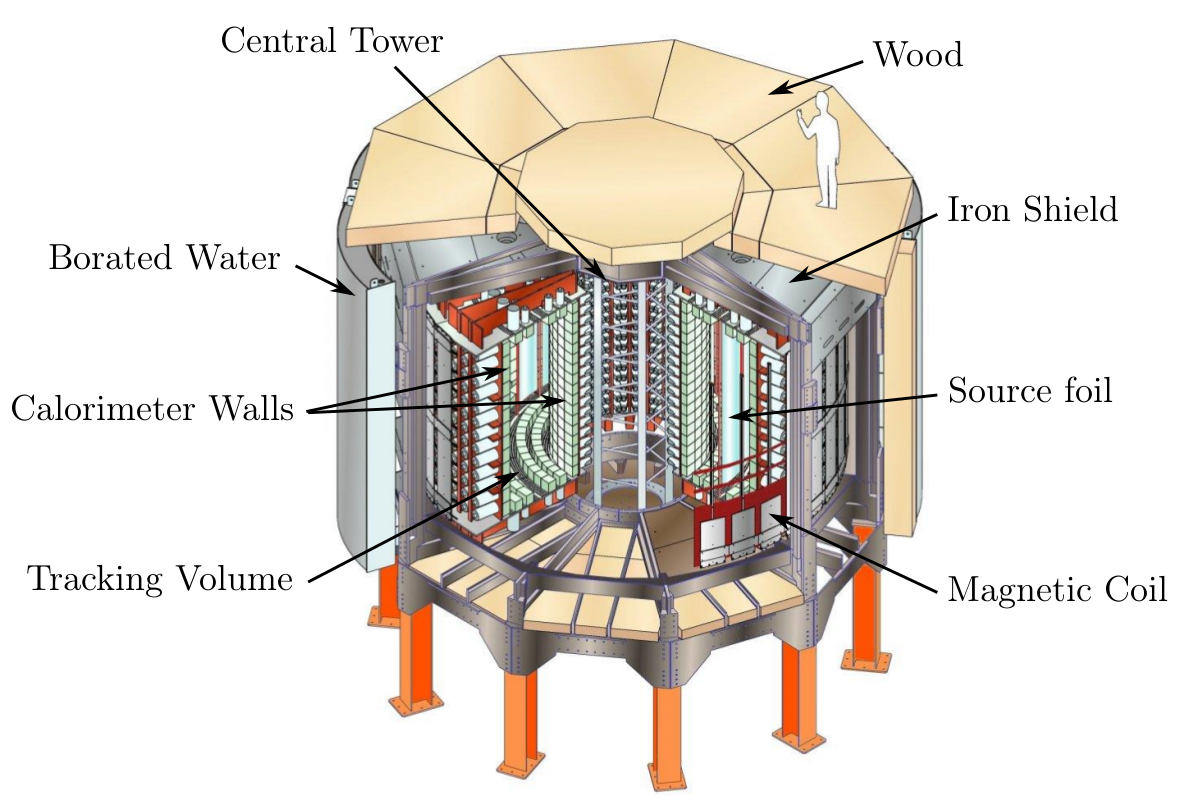
\includegraphics[scale=0.35]{pictures/Chap2/NEMO-3-Schema.png}
\caption{Exploded view of the NEMO-3 detector.}
\label{NEMO3Detector}
\end{center}
\end{figure}

\begin{figure}[h!]
\begin{center}
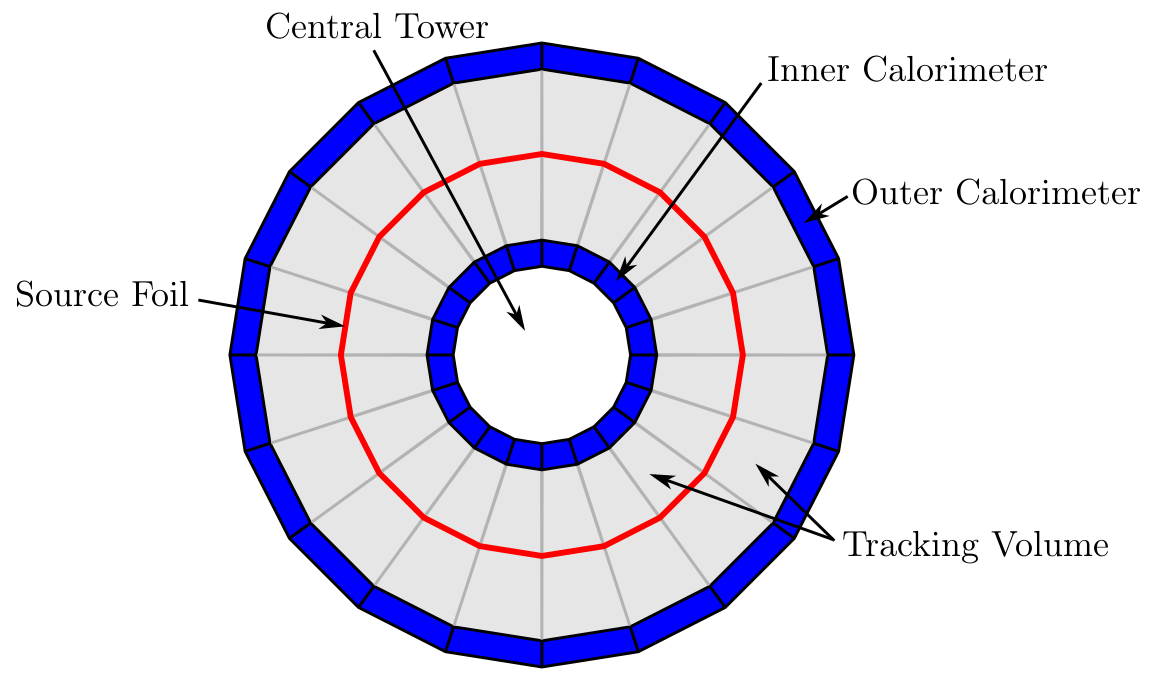
\includegraphics[scale=0.35]{pictures/Chap2/TopViewNEMO3.png}
\caption{Top view of the~NEMO-3~detector geometry. The $\beta\beta$ source foils are represented in red, the tracker volume in grey and the calorimeter in blue. The cylinder is divided into 20 sectors.}
\label{TopViewNEMO3}
\end{center}
\end{figure}

\begin{figure}[h!]
\begin{center}
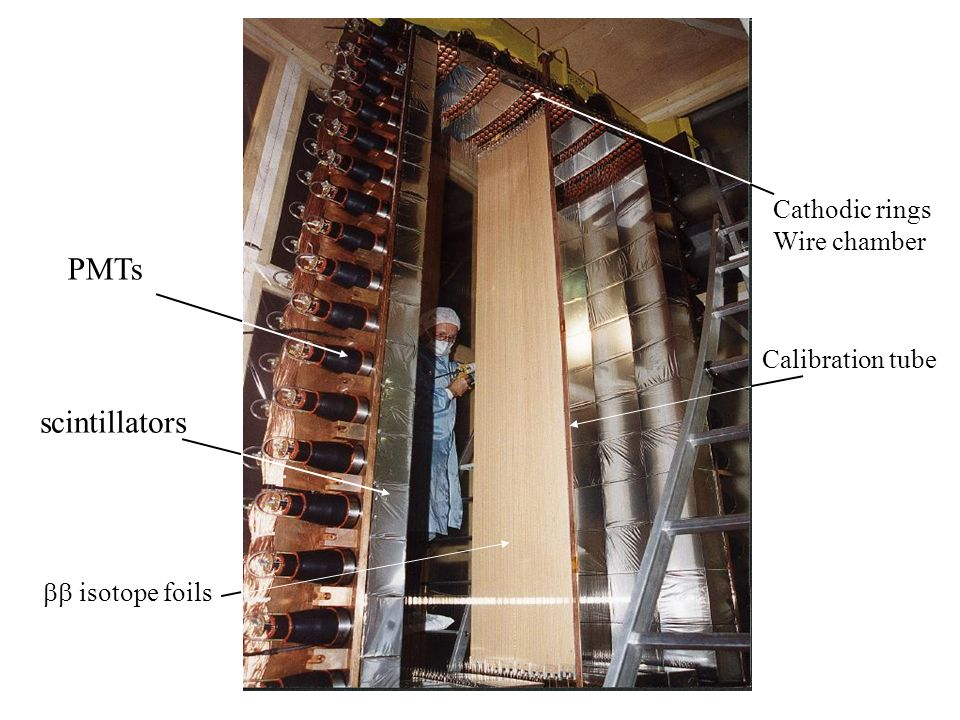
\includegraphics[scale=0.65]{pictures/Chap2/sector.jpg}
\caption{Picture of a NEMO-3 sector. A source foil is verticaly placed at the center and surrounded by the wire chamber and the calorimeter.}
\label{NEMO3SectorPictures}
\end{center}
\end{figure}


\FloatBarrier


\subsection{Source foils}


\NI The separation of the source foils from the rest of the detector allows the investigation of various $\beta\beta$ emitters. Seven isotopes for a total of 8.8~kg have been introduced in the detector. $^{\text{100}}$Mo and $^{\text{82}}$Se were the isotopes with the largest mass with 6.91~kg and 0.93~kg respectively. These two isotopes provide the best sensitivity to search for 0$\nu\beta\beta$ decays. Smaller quantities have been included to investigate 0$\nu\beta\beta$ and measure the 2$\nu\beta\beta$ decay rate, including 0.45~kg of $^{\text{130}}$Te, 0.40~kg of $^{\text{116}}$Cd, 36.6~g of $^{\text{150}}$Nd, 9.43~g of $^{\text{96}}$Zr, and 6.99~g of $^{\text{48}}$Ca. Alongside the enriched foils, 0.6~kg of very pure natural tellurium and 0.6~kg of ultra-pure copper foils were installed to control and validate the background measurements. The distribution of the isotopes around the 20 sectors are shown in Figure~\ref{NEMO3Sector}. The masses, Q$_{\beta\beta}$ values, and natural abundances ($\eta$) for each of these $\beta\beta$ isotopes are given in Table~\ref{tab:isotopeNEMO3}.



\begin{figure}[h!]
\begin{center}
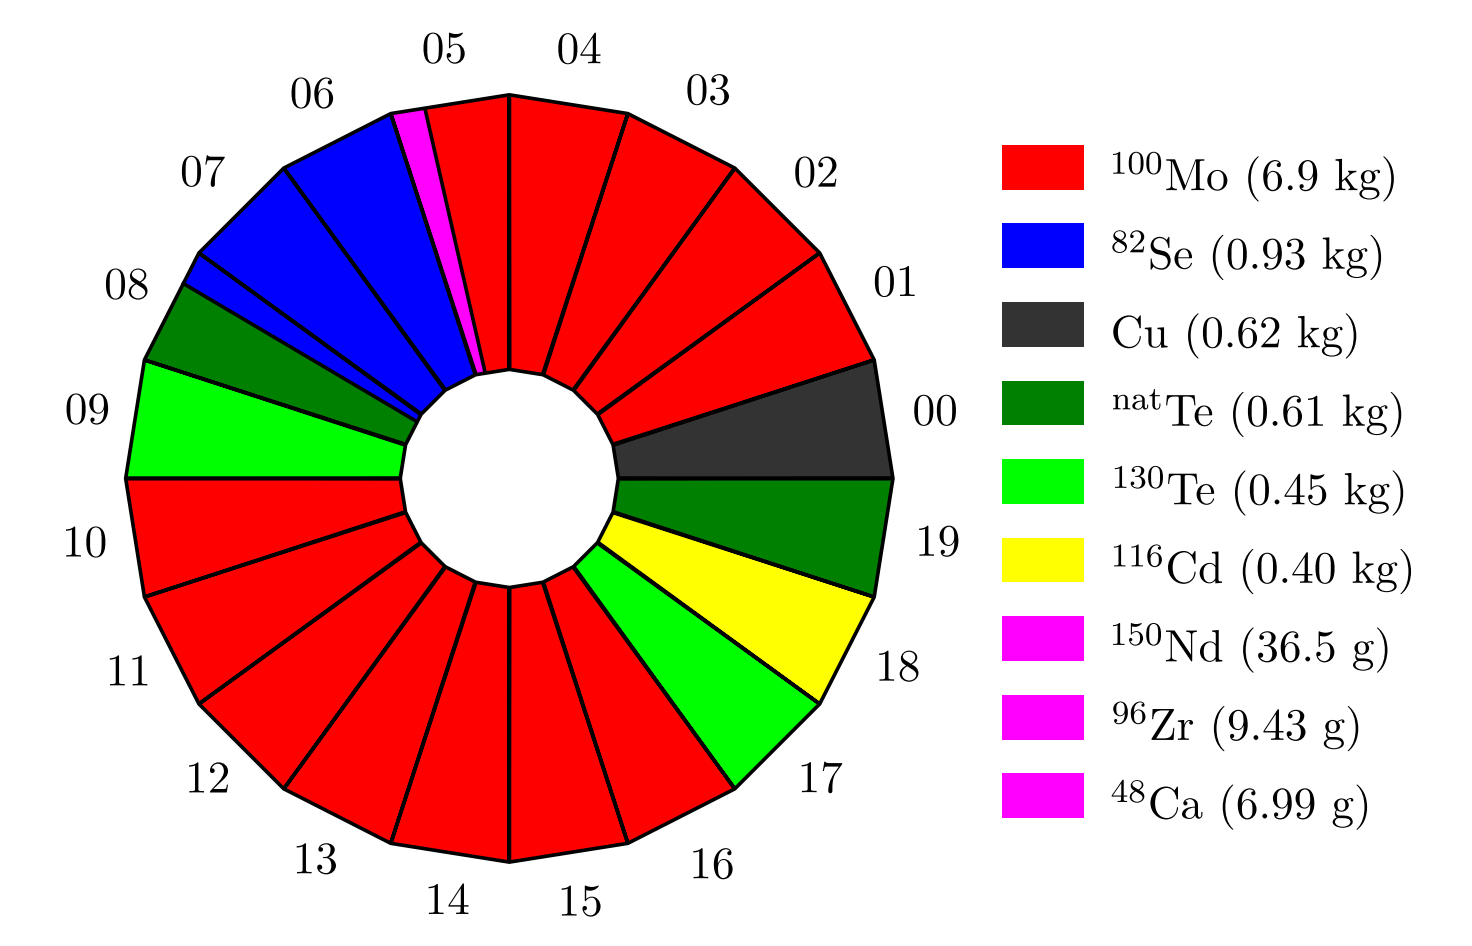
\includegraphics[scale=0.5]{pictures/Chap3/BBSourceDistribution.png}
\caption{Schematic view of the seven different $\beta\beta$ sources location inside the NEMO-3 detector. The main isotopes was $^{\text{100}}$Mo (6.9~kg) and $^{\text{82}}$Se (0.9~kg).}
\label{NEMO3Sector}
\end{center}
\end{figure}



\NI Each sector supports a source frame with seven strips of $\beta\beta$ emitter 248~cm~long. The five central strips were  6.5~cm wide, while the two strips on the edge were 6.3~cm wide. The surface density of the strips are in the range 30~-~60~mg/cm$^\text{2}$, which is a compromise to maximise the isotope mass while maintaining the foil thin enough to reduce the electron multiple scatterings through the foil bulk, and to not degrade the energy resolution.


\bigskip


\NI Two different sorts of sources were in NEMO-3~: metallic and composite. The metallic sources are metallic foils having a density of approximately 10~g/cm$^\text{3}$, corresponding to a thickness of 60~$\mu$m. The $^{\text{116}}$Cd, part of $^{\text{100}}$Mo and the copper foils were metallic. Note that the $^{\text{116}}$Cd foils were wrapped into a plastic film to avoid them to creep. The composite foils are a mixture of source powder and organic glue. The density of the composite foil were approximately five times lower than the metallic foils, allowing thickness up to 300~$\mu$m. The composite foils were surrounded by two mylar films to provide mechanical strength. To ensure a good bond with the glue and facilitate evaporation, the mylar sheets have a large number of microscopic holes. The $^{\text{82}}$Se, $^{\text{130}}$Te, $^{\text{96}}$Zr, $^{\text{150}}$Nd and $^{\text{48}}$Ca and a part of $^{\text{100}}$Mo foils were composite.



%\begin{table}[h!]
%\centering
%\begin{tabular}{c|c|c|c|c}
%Isotopes & Mass [g] & Q$_{\beta\beta}$ [MeV] & T$_{\text{1/2}}^{\text{2}\nu}$ [y] & Abundance [\%]\\[0.05cm]
%\toprule
%$^{\text{100}}$Mo & 6 914 $\pm$ 22    & 3.034 $\pm$ & 7.2 $\times$ 10$^{\text{18}}$ & 9.63 $\pm$ \\[0.1cm]
%$^{\text{82}}$Se  & 932   $\pm$ 5     & 2.995 $\pm$ & 9.6 $\times$ 10$^{\text{19}}$ & 8.73 $\pm$ \\[0.1cm]
%$^{\text{130}}$Te & 454   $\pm$ 2     & 2.529 $\pm$ & 7.0 $\times$ 10$^{\text{20}}$ & 33.8 $\pm$ \\[0.1cm]
%$^{\text{116}}$Cd & 410   $\pm$ 1     & 2.802 $\pm$ & 2.9 $\times$ 10$^{\text{19}}$ & 7.49 $\pm$ \\[0.1cm]
%$^{\text{150}}$Nd & 37    $\pm$ 0.1   & 3.367 $\pm$ & 9.1 $\times$ 10$^{\text{18}}$ & 5.6  $\pm$ \\[0.1cm]
%$^{\text{96}}$Zr  & 9.4   $\pm$ 0.2   & 3.350 $\pm$ & 2.4 $\times$ 10$^{\text{19}}$ & 2.8  $\pm$ \\[0.1cm]
%$^{\text{48}}$Ca  & 6.99  $\pm$ 0.05  & 4.271 $\pm$ & 4.4 $\times$ 10$^{\text{19}}$ & 0.19 $\pm$ \\[0.1cm]
%\bottomrule
%\end{tabular}
%\caption{Mass, Q$_{\beta\beta}$, T$_{\text{1/2}}^{\text{2}\nu}$ and abundance of the different isotopes introduced in NEMO-3.}
%\label{tab:isotopeNEMO3}
%\end{table} 

\begin{table}[h!]
\centering
\begin{tabular}{c|c|c|c}
\toprule
Isotopes & Mass [g] & Q$_{\beta\beta}$ [keV] & $\eta$ [\%]\\[0.05cm]
\hline
$^{\text{100}}$Mo & 6 914 $\pm$ 22    & 3034.40 $\pm$ 0.17 & 9.63 \\[0.1cm]
$^{\text{82}}$Se  & 932   $\pm$ 5     & 2997.9  $\pm$ 0.3  & 8.73 \\[0.1cm]
$^{\text{130}}$Te & 454   $\pm$ 2     & 2528.9  $\pm$ 2.1  & 33.8 \\[0.1cm]
$^{\text{116}}$Cd & 410   $\pm$ 1     & 2813.50 $\pm$ 0.13 & 7.49 \\[0.1cm]
$^{\text{150}}$Nd & 37    $\pm$ 0.1   & 3371.38 $\pm$ 0.20 & 5.6  \\[0.1cm]
$^{\text{96}}$Zr  & 9.4   $\pm$ 0.2   & 3350.0  $\pm$ 3.5  & 2.8  \\[0.1cm]
$^{\text{48}}$Ca  & 6.99  $\pm$ 0.05  & 4267.98 $\pm$ 0.32 & 0.19 \\[0.1cm]
\bottomrule
\end{tabular}
\caption{Mass, Q$_{\beta\beta}$, T$_{\text{1/2}}^{\text{2}\nu}$ and natural abundance of the different isotopes introduced in NEMO-3.}
\label{tab:isotopeNEMO3}
\end{table} 


\subsection{The \texorpdfstring{\Cd}~ source foil}
\label{sec:CdSectorInNEMO3}


\NI A total mass of 440~g of cadmium was placed in sector 18. The average enrichment of \Cd~was (93.2~$\pm$~0.2)\%~\cite{NEMO-3-detector} which represents an effective mass of (410~$\pm$~1)~g~of~\Cd. The enrichment has been realized by the centrifugation separation method. Despite the good yield of this technique, smaller amounts of other cadmium isotopes are still present in the sample, see Table~\ref{tab:IsotopeCdTable}. Part of the sample (152~g) was previously measured with the NEMO-2 prototype~\cite{ObservationCd116NEMO-2}.  


\bigskip


\NI The cadmium has been divided in seven~strips of 2423~cm long and $\sim$~6.5~cm wide. Each strip was made of one or more smaller pieces which were glued together with Araldite~AW~106 and a hardener~HV953V. Two 12-$\mu$m mylar films surrounded the entire strip to provide mechanical strength. The mylar films were glued using Araldite~2020/A~XW~3961 and Araldite~2020/B~XW~3972.


\begin{table}[h!]
\begin{center}
\begin{tabular}{c|c|c}
\toprule
Isotope & Mass fraction & Mass (g) \\
\hline
116   & 0.932   & 410.08 \\[0.05cm]
114   & 0.03228 & 14.20  \\[0.05cm]
113   & 0.00885 & 3.90   \\[0.05cm]
112   & 0.01544 & 6.79   \\[0.05cm]
111   & 0.00535 & 2.35   \\[0.05cm]
110   & 0.00468 & 2.06   \\[0.05cm]
108   & 0.00032 & 0.14   \\[0.05cm]
106   & 0.00038 & 0.17   \\[0.05cm]
Total & 0.999   & 439.69 \\[0.05cm]
\bottomrule
\end{tabular}
\end{center}
\caption{Isotopes present in the 440~g of Cd sample placed in NEMO-3 detector. The total mass of \Cd~is (410~$\pm$~1)~g which takes into account the error on the enrichment yield of 0.2\%.}
\label{tab:IsotopeCdTable}
\end{table}


\bigskip


\NI To ensure a good bond with the glue, the mylar sheets were perforated of microscopic holes of around 0.4 $\mu$m in diameter. The perforation has been realized at the Joint Institute for Nuclear Research (JINR, Dubna, Russia) by irradiating the mylar with a $^{\text{84}}$Kr ion beam of 3~MeV/nucleon at a luminosity of 5~$\times$~10$^{\text{11}}$ ions/s. The mylar was chemically etched with NaOH at 70$^{\circ}$~C, washed with water and 1~\% of acetic acid. Finally, the film was dried with hot air. All the materials entering in the process of the backing film have been selected for their radio-purity and have been measured with High Purity Germanium detectors at LSM.


\bigskip


\NI Each strip was connected to their neighboring strips with glue (Araldite~AW106). A schematic view of the~seven~cadmium foils in sector~18 is shown in~Figure~\ref{CdFoil}. After the installation, some gaps ranging from 2~mm to 4~mm between some parts of the strips have been observed. The source shape is not strictly cylindrical as shown in the top section of~Figure~\ref{CdFoil}. It was also found that straining of the strips was small due to the softness of the cadmium metal~\cite{SoftnessCdMetal}. 


\bigskip


\begin{figure}[h!]
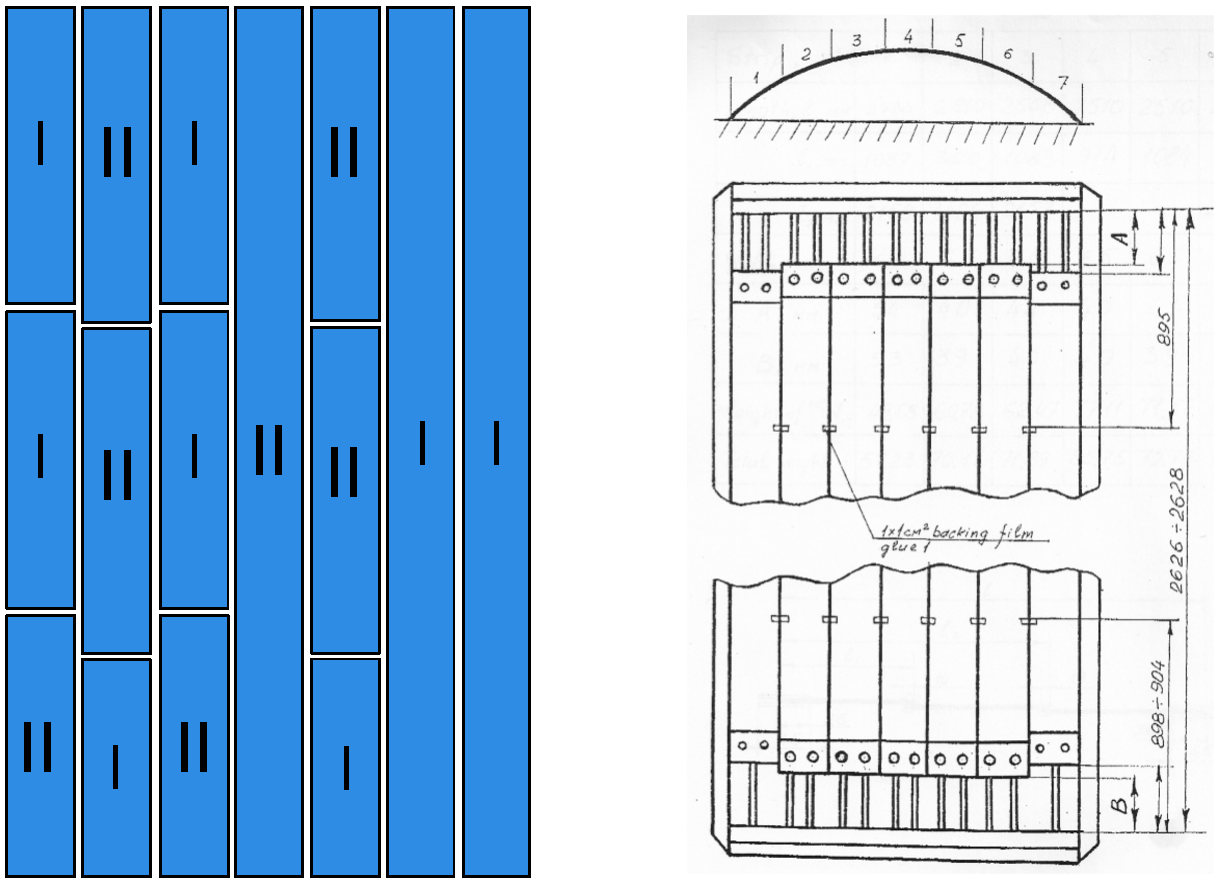
\includegraphics[height=7.7cm]{pictures/Chap6/schemaFoil_v2.pdf}
\centering
\caption{Left : Schematic view of the sector 18. The seven cadmium foils are divided in smaller pieces and glued together. The labels I and II correspond to the different \Cd~productions. Right : Drawing of the strips of cadmium showing the plexiglass clips that attach the foil to the support structure. Small pieces of backing film were used to join the individual strips to one another.}
\label{CdFoil}
\end{figure}


\NI Before being introduced in the detector, the radioactive contaminations of the cadmium foils have been measured thanks to High Purity Germanium detector (HPGe). The results of the different contaminations are summarized in Table \ref{TableContaminationMeasurements}.


\bigskip


\begin{table}[h!]
\begin{center}
\begin{tabular}{c|c|c|c|c|c|c|c|c}
   \toprule
   Source  & Mass [g] & Exposure [h] &\multicolumn{6}{c|}{Activity [mBq/kg]} \\
   \hline
           &          &              & $^{\text{40}}$K &  $^{\text{235}}$U &  $^{\text{234}}$Th & $^{\text{214}}$Bi  & $^{\text{228}}$Ac & $^{\text{232}}$Tl \\[0.1cm]
   Type I  & 257      & 778          & < 13     & < 0.5      & < 12        & < 1.5                  & < 2        & < 0.5 \\
   Type II & 299      & 368          & < 20     & < 1        & < 56        & < 1.7                  & < 4        & < 0.83 \\
   \bottomrule
\end{tabular}
\caption{Measurements of the cadmium source foils (including mylar support) realized with HPGe detector.}
\label{TableContaminationMeasurements}
\end{center}
\end{table}


\FloatBarrier


\subsection{Tracker}


\NI The NEMO-3 tracker provides three-dimensional tracking of charged particles to measure the decay properties of $\beta\beta$ events. It is composed of 6180 vertical drift cells operating in Geiger mode, which surround the source foils on both sides. The cells are arranged into nine different layers and divided into a 4-2-3 configuration, as shown in Figure~\ref{TrackerNEMOView}. The four layers close to the source allow a good reconstruction of the $\beta\beta$ vertex location to the source foil, the two middle layers provide the measurement of the track curvature and the three final layers are used to determine the interaction point of the calorimeter block. The gaps between the layers correspond to the location of calorimeter modules on top and bottom, which increase the coverage of the detector.


\bigskip


\begin{figure}[h!]
\begin{center}
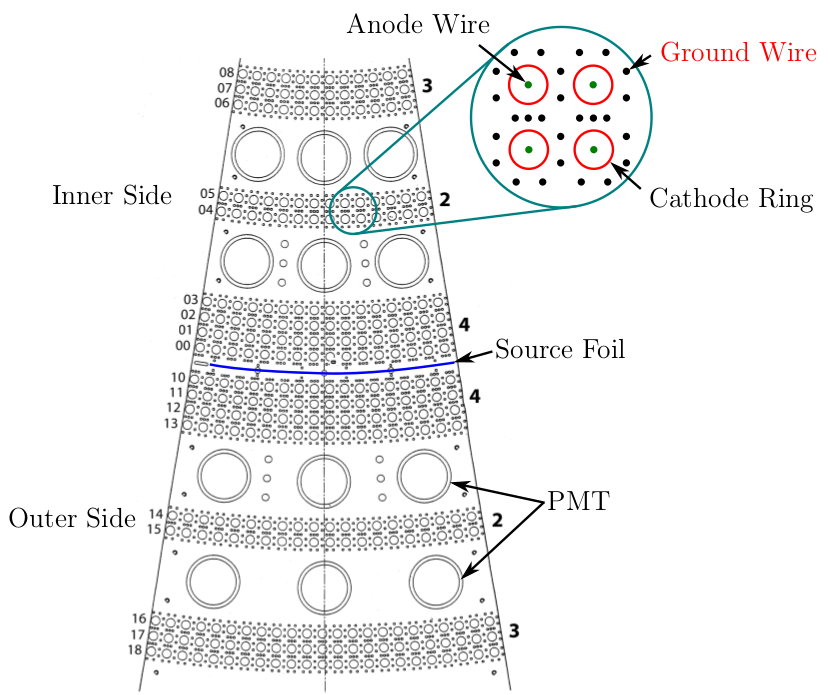
\includegraphics[scale=0.30]{pictures/Chap3/TrackerNEMOview.png}
\caption{Left : The 4-2-3 configuration of the Geiger cells in a NEMO-3 sector The 12 large rings represent the location of the light guides installed in the support structure to couple the scintillators to the PMTs. Right : Geiger
wiring of four elementary Geiger cells.}
\label{TrackerNEMOView}
\end{center}
\end{figure}


\NI An elementary cell, shown in Figure~\ref{GeigerCellNEMO3}, is 2.7~m long and 3~cm in diameter, consisting of a central anode wire surrounded by eight ground wires. Four of these cathode wires are shared between the neighbouring cells, as shown in Figure~\ref{TrackerNEMOView}. This is an advantage from a radiopurity point of view because it reduces the amount of material in the tracker volume. It also minimizes the scattering inside the tracker. An extra ground wire has been added between the layers to avoid electrostatic cross talk. The wires are made of stainless steel, 2.7~m long and 50~$\mu$m in diameter. Copper cathode rings located at the top and bottom of the anode wires collect signals. These rings are 3~cm long and 2.3~cm in diameter.


\bigskip


\NI The gas inside the tracker volume is a mixture of 95~\% of helium, 4~\% of ethanol, 1~\% of argon and 0.1~\% of water held at 10~mbar above atmospheric pressure. Helium is used as basis of the tracking gas, since it is a noble gas with a low atomic number, which minimises multiple scatterings. When traversing the tracker, an electron from $\beta\beta$ decay loses only approximately 30~keV. Small quantities of ethanol are used to quench the photoionisation process, by absorbing UV photons. The performance of the tracker is then improved by reducing the re-firing effect of one cell to another. Some argon is also introduced to the mixture to stabilize the plasma propagation. Finally, in the final year of the detector, very small amounts of water vapour have been added in order to rejuvenate the ageing cells.



\begin{figure}[h!]
\begin{center}
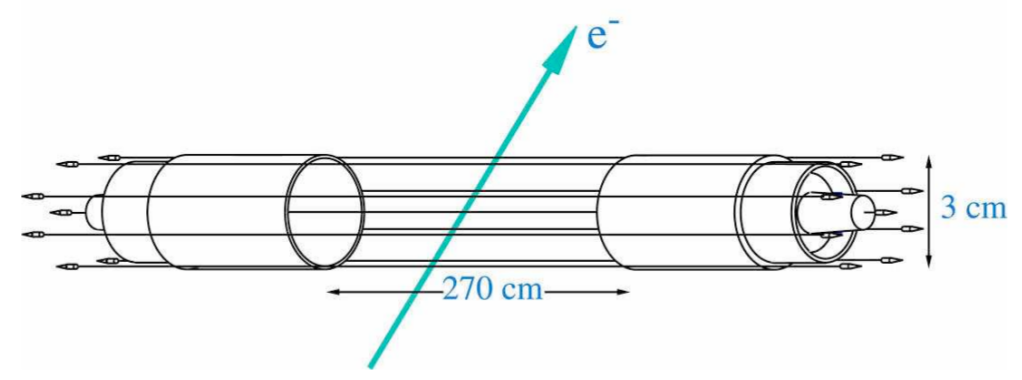
\includegraphics[scale=0.3]{pictures/Chap3/GeigerCellNEMO3.png}
\caption{Representation of an elementary Geiger cell in NEMO-3. The central anode wire of 270~cm length is surrounded by 8 ground wires. The cathode rings are shown at each end of the cell, 3~cm of diameter.}
\label{GeigerCellNEMO3}
\end{center}
\end{figure}


\NI When a charged particle crosses the tracking volume, the gas is ionized, producing He$^{+}$ ions and electrons. By applying a potential difference of about 1600~V between anode and cathode wires, these electrons drift towards the central anode and are accelerated, ionising more atoms. This creates an avalanche that arrives at the anode wire and produces a signal. In this operating mode, a crossing charged particle creates $\sim$~6~electrons/cm. The drift speed is $\sim$~2.3 cm/$\mu$s, close to the anode, and $\sim$~1~cm/$\mu$s near the ground wires. The radial position of a particle can be reconstructed using the drift time and the globlal trigger (see Section~\ref{sec:triggerAndDAQ}). During the electron avalanche, induced UV photons create a plasma that propagates along the length of the wire at a speed of $\sim$~6 to 7 cm/$\mu$s. The detection of this plasma by the cathode rings on both sides gives information on the longitudinal position of a crossing particle. For 1~MeV electron, the average hit resolution of a cell has been measured to be 0.5~mm on the transversal plane and 8.0~mm on the longitudinal axis.


\subsection{Calorimeter}


\NI The role of the NEMO-3 calorimeter is to measure the energy of the incident particles, to provide timing information of particles in an event, and to provide a fast trigger signal. The calorimeter surrounds the tracking chambers on all sides. It consists of 1940 separated optical modules. Each optical module is made of a scintillator block, two light guides and a PMT. A schematic view of a NEMO-3 optical module is presented in Figure~\ref{CaloModuleNEMO3}.	


\bigskip

\begin{figure}[h!]
\begin{center}
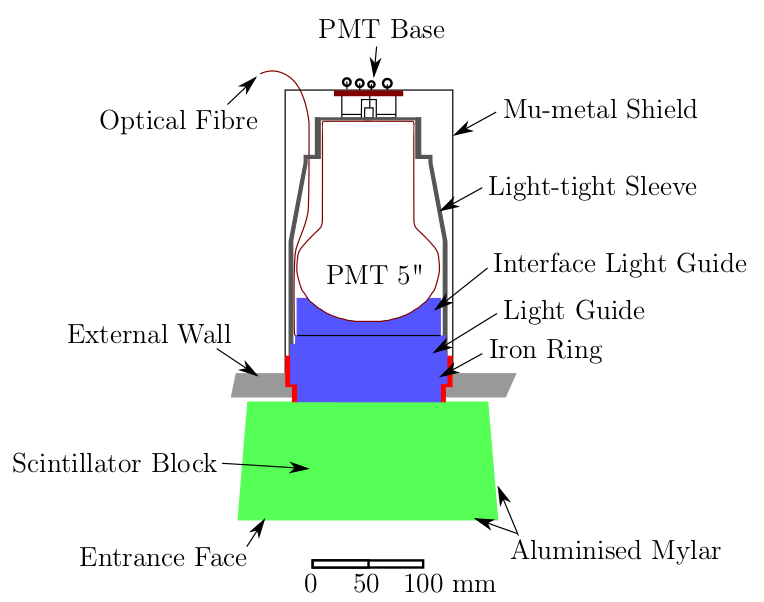
\includegraphics[scale=0.40]{pictures/Chap3/CaloModuleNEMO3.png}
\caption{Schematic of a single NEMO-3 calorimeter module.}
\label{CaloModuleNEMO3}
\end{center}
\end{figure}


\NI The scintillator blocks are made of a polystyrene, (C$_\text{6}$H$_\text{5}$CH=CH$_\text{2}$), doped with a scintillating agent, p-Terphenyl (PTP), and a wavelength shifter 1.4-di-(5-phenyl-2-oxazoly) benzene (POPOP). By entering a block, charged particles lose their energy through ionization and excite molecules with an energy proportional to the deposited energy. During its de-excitation, PTP translates energy into scintillation light. This light is then shifted by POPOP into a wavelength matching to the PMT sensitivity. The scintillation light is carried to the PMT via 60~mm thick light guides made of polymethyl methacrylate (PMMA). The light transmission through the guides is approximately 98~\%. These light guides also provide a protection for the PMT against the helium of the tracker gas, which would damage the PMTs. The four lateral sides of the scintillator block are wrapped with 350~$\mu$m of polytetrafluoroethylene (PTFE) in order to diffuse scintillation light and increase overall collection. A 12~$\mu$m layer of aluminised Mylar covers the blocks to increase light collection and protect the scintillator from UV photons produced inside the tracker.


\bigskip


%\NI The detection of the $\gamma$-ray is based on the same mechanism as electron detection. But, due to the low density of the plastic scintillator block, the $\gamma$-rays, in a range of interast for the NEMO-3 experiment (0.2 - 10.0~MeV), mainly interact by Compton scattering. The total energy of the $\gamma$-ray may not be recorded within a single module since only the energy of the scattered electron is measured. An algorithm have been developed to cluster neighbour scintillator hits to allow a more accurate reconstruction of the $\gamma$-ray energy.


\bigskip


\NI To fit the cylindrical geometry of NEMO-3, there are seven different block types referred to as IN, EE, EC, and L1-L4. The location of these blocks is shown in Figure~\ref{SectorDetailedPMTconfig}. The EE and EC blocks are located on the outer calorimeter wall and are coupled to 5'' PTMs. The IN blocks corresponds to the blocks located on the inner calorimeter wall and are coupled to 3'' PMTs. The L1, L2, L3 and L4 blocks are called petal blocks. They are located on the top and bottom of the detector, L1 being the blocks closest to the inner wall and L4 being the blocks closest to the outer wall. They are coupled to 3'' PMT except L4 ones which are coupled to 5'' PMT.  


\begin{figure}[h!]
\begin{center}
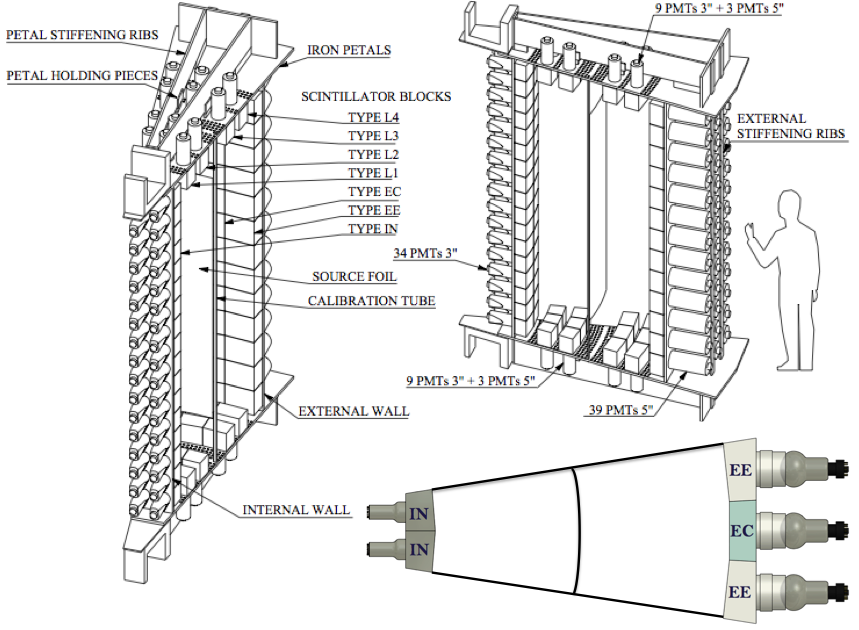
\includegraphics[scale=0.34]{pictures/Chap3/SectorDetailedPMTconfig.png}
\caption{One sector of NEMO 3 with details on the source foil, scintillator blocks and photomultipliers location.}
\label{SectorDetailedPMTconfig}
\end{center}
\end{figure}


\NI The composition and the size of the scintillator blocks are not the same, depending on their position in the detector. The IN, EE and EC blocks are made of 98.49~\% of polystyrene, 1.5~\% of PTP, and 0.01~\% of POPOP. The IN blocks are the smallest with a front face size of 153~$\times$~154 mm. The EE and EC are the largest with a front face sizes of 200~$\times$~218~mm. All the petal blocks are made of 98.75 \% of polystyrene, 1.2~\% of PTP, and 0.05~\% of POPOP. The L1 blocks have a similar size to the IN blocks and L4 have similar size to the EE blocks. 


\bigskip


\NI The Hamamatsu company was chosen to produce the 3'' and 5'' PMTs. The 3'' PMTs (R6091) possess twelve dynodes and a flat photocathode, while the 5'' (R6594) have ten dynodes and hemispherical photocathode. The radiopurity of the PMT glass has been measured by HPGe detector. The contamination in $^{\text{40}}$K, $^{\text{214}}$Bi and $^{\text{208}}$Tl have been found to be 0.34~Bq/PMT, 0.083~Bq/PMT and 5$\times$10$^{\text{-3}}$~Bq/PMT, respectively, for the 3'' PMTs, and 0.53~Bq/PMT, 0.24~Bq/PMT and 0.014 Bq/PMT for the 5'' PMTs.


\FloatBarrier


\subsection{Trigger and DAQ}\label{sec:triggerAndDAQ}


\NI The NEMO-3 detector has independant tracker and calorimeter electronics and data acquisition systems. This separation allows individual or interdependant triggering and data readout to operate in different configurations. 


\bigskip


\NI The 1940 PMTs of the calorimeters was supplied at 1800~V (3'') and 1350~V (5'') with three CAEN power supplies. Each power supply is able to provide 240~HV channels. The anode wires of the NEMO-3 tracker are supplied at a level of 1620-1650~V thanks to two CAEN power supplies. 


\subsubsection{Trigger system}


\NI The trigger system of NEMO-3 has three separate levels referred to as T1, T2 and T3. T1 is based on informations given by the calorimeter. A low and high thresholds are set in the electronic boards which read-out data from the PMTs. In case a PMT exceeds the lower threshold, which is set at 7~mV (or 23~keV equivalent), a TDC measurement and charge integration window of 80~ns opens. If a PMT exceeds the high threshold, which is set at 48~mV (150~keV), a signal is sent to the trigger logic. As a consequence, a STOP-PMT signal is sent to all calorimeter channels that stops TDC measurements and stores the integrated charge recorded in each PMT. This STOP-PMT signal is used as the time reference for the event.


\bigskip


\NI T2 is based on information given by the tracker. After the STOP-PMT signal, the read-out electronics for Geiger cells is activated during 6.14~$\mu$s. If an anode pulse coming from a single cell occurs within this time window, this cell is labelled as prompt hit and initiates the TDC measurements for this cell. In the same time, a HIT-GG signal is sent for all Geiger cells in its layer. The stop signal for TDC is provided when the Geiger plasma reaches the cathode rings. To meet the T2 requirements, at least three of the nine Geiger layers must be hit within a half-sector, and two of the hits must be in neighbouring layers.


\bigskip


\NI The event read-out is initiated if both T1 and T2 requirements are met. The digitized time and signal for the triggered PMT channels are read out with two 14-bit analog-to-digital converters (ADCs). After the STOP-PMT signal, the Geiger cells which are not triggered within the 6.14~$\mu$s window continue the data collection up to 710~$\mu$s. The TDC information of the delayed Geiger hits arriving in this time window is read out and stored. This information are then used to idenfy the Bi-Po cascade events.


\bigskip


\NI T3 is only used during the calibration runs. It combines informations from T2 with information from the calorimeter to select events likely to come from radioactive sources.




\subsection{Energy and time calibration}\label{sec:EnergyTimeCalibration}


\NI As the electron energy is one of the most effective means to discriminate 0$\nu\beta\beta$ signal from background, the calorimeter performance variations must be monitored over the life time of the experiment. The absolute energy and time calibration was performed every $\sim$~40 days in dedicated runs. The stability of the detector between these runs was ensured by daily laser surveys.
  

\subsubsection{Calibration sources}


\NI To calibrate the absolute energy, $^{\text{207}}$Bi sources were introduced into the detector via copper calibration tubes located at the boundaries between each sector, and at the same radius as the source foil. Each calibration tube was equipped with three pairs of kapton windows, faced towards the inner and outer calorimeter walls, to allow for calibration source products to exit the tubes with minimal scattering. The vertical positions of the windows were at z~=~-90, 0 and +90~cm in order to maximise the illumination uniformity of the scintillator blocks. The decay of $^{\text{207}}$Bi produces two conversion electrons with energies of 482~keV and 976~keV. The comparison between the ADC response from each of the PMTs and these known electron energies provide two-point energy calibration reliable up to 1.5~MeV. To calibrate up to 3~MeV, a $^{\text{90}}$Sr calibration source was used. The end-point of the $\beta$-decay spectrum of its daughter, $^{\text{90}}$Y, is at 2.28~MeV. The matching of ADC values to this end-point provide a third data point to calibrate the energy.


\bigskip


\NI Tests during the assembly of the optical module observed a dependance of the energy response according to the impact point on the scintillator block. The effect observed may be as large as 10~\% for the 5'' PMTs. By combining multiple $^{\text{207}}$Bi runs it is possible to apply corrections to the energy response based on the impact point with the scintillator.


\bigskip


\NI The $^{\text{207}}$Bi sources are also used to derive the calorimeter energy resolution. By fitting the two conversion electron peaks with multiple Gaussian functions, the energy resolution is extracted from the FWHM. For 1~MeV electrons, the FWHM is found to be~14-17~\%. 
 
 
\bigskip


\NI To calibrate the time response of the calorimeter, $^{\text{60}}$Co sources were used. This isotope decays via simultaneous emissions of two $\gamma$-rays with energies of 1173~keV and 1332~keV~\cite{DecayCo60}. Knowing the distance between each calorimeter blocks and the source position, the difference in arrival time between the two $\gamma$-rays is used to measure the relative time shifts between each channel. The $^{\text{60}}$Co sources are moved to several different positions to cover entirely the detector and all possible combinaisons of PMTs.


\bigskip


\NI To determine the timing resolution, for 1~MeV electrons, the difference in arrival time between the two electrons from $^{\text{207}}$Bi is used. It has been found to be $\sigma_{\text{t}}$ = 250~ps~\cite{NEMO-3-detector}.

 
\subsubsection{Laser survey}


\NI To monitor the stability of the calorimeter between absolute calibration runs, a laser calibration system has been developed. A di-azote laser (N$_\text{2}$) with a wavelength of 337~$\pm$~15~nm is used. The light beam is divided into two parts. The first is directly sent to a photocathode to monitor the laser light intensity. The second beam is shifted to 420~nm using a small spherical scintillator to mimic an electron signal. This signal is sent to the NEMO-3 calorimeter blocks via optical fibers. The light is also sent to six reference PMTs equipped with $^{\text{207}}$Bi, allowing to monitor the laser intensity by measuring energies of both the laser and the 976 keV conversion electrons.


\bigskip


\NI After each absolute calibration run, a laser survey is immediately conducted, and constitutes a reference position for the laser light peak (C$^{\text{t}_\text{0}}_{\text{laser}}$) in the reference PMTs and calorimeter PMTs. A second reference point is determined for the reference PMT, by comparing C$^{\text{t}_\text{0}}_{\text{laser}}$ to the 976~keV electron from the $^{\text{207}}$Bi source (C$^{\text{t}_\text{0}}_{\text{Bi}}$). The shift of the laser peak over the time (C$^{\text{t}}_{\text{laser}}$) is monitored for all PMTs. Any changes in C$^{\text{t}}_{\text{laser}}$ reflects both a change in the NEMO-3 PMT performances and changes in the laser light itself. By comparing C$^{\text{t}}_{\text{laser}}$ to C$^{\text{t}_\text{0}}_{\text{Bi}}$, the consequences from a change in the laser light are calibrated out, leaving only the gain variation in the PMTs to account for.


\bigskip


\NI In case a PMT fluctuates too much over time, it is removed from the analysis for the periods of instability. It has been found that there is no instability for 87~\% of the PMTs, with a further 7~\% being unstable in a brief period.

\subsection{Magnetic coil and shielding}


\NI Despite the fact that NEMO-3 was located at LSM under 4800~m.w.e, which highly reduces the cosmic muon flux, the detector must be protected from different background sources. Neutrons produced from ($\alpha$, n) reactions, cosmic muon spallation or spontaneous fission of uranium undergo neutron capture and produce high energy $\gamma$-rays. As seen in Section~\ref{sec:MinimisingBkg}, these $\gamma$-rays are able to reproduce the $\beta\beta$ decay signal. Layers of passive shielding were installed around the detector to protect against the external neutron and $\gamma$-ray flux. A magnetic field allowing for positron/electron discrimation helps the identification of remaining external decay products.


\subsubsection{The magnetic coil}


\NI A solenoid magnet surrounding entirely the calorimeter produces a magnetic field of 25~Gauss parallel to the axis of the cylinder. The field is generated by running a current of $\sim$~ 30~A through a 5~tons copper coil of 5320 mm in diameter, 2713 mm high. Fans were used to cool the coil and the PMTs. A $\mu$-metal shielding is used to protect the PMTs from the magnetic field. 


\bigskip


\NI The magnetic field allows discrimination between $\beta\beta$ decay events and electron-positron (e$^+$e$^-$) pair from interactions of high energy $\gamma$-rays in the source foil. The rejection efficiency of e$^+$e$^-$ pair is $\sim$~95~\% at 1~MeV~\cite{NEMO-3-detector}. 

\bigskip


\subsubsection{The shieldings}


\NI To suppress the neutron flux inside NEMO-3, a neutron shielding surrounds the detector. This shield consists of 20~cm of paraffin located below the central tower (not shown in Figure~\ref{NEMO3Detector}), 35~cm of borated water placed in tanks and 28~cm of wood above and below the detector end caps. Neutrons are thermalized by the paraffin, wood or water, and captured on boron. 


\bigskip

\NI To stop the $\gamma$-ray emitted in the neutron capture, a second shield made of iron is placed between the detector and the first shielding. This shield is made of 177 tonnes of iron, selected for its radiopurity, and is 20~cm thick.


\subsubsection{The anti-radon facility}


\NI Despite precautions taken to isolate the detector from the laboratory air with radon-tight seals, an excess of radon has been discovered after one year of data-taking. This high level of radon was due to leaks through the joints of the external shielding and calorimeter walls.


\bigskip


\NI To fix this problem, an anti-radon facility has been installed at the end of 2004. The facility is made of an hermetic polyethylene tent surrounding the entire detector, filled by radon-free air. The air of the laboratory was purified thanks to a radon trapping system using porous charcoal. When the air passes through the charcoal, the radon is trapped for a period of time allowing its decay. The output air is three orders in magnitude poorer in radon than the incoming air.


\bigskip


\NI After the installation of the anti-radon facility, the level of radon inside NEMO-3 decreased by a factor $\sim$~6~\cite{NEMO3-BKG}, see Figure~\ref{RadonByTime}. This reduction is much lower than the expected reduction, which is not completely explained. The two main hypotheses are that there is a higher radon level inside the tent than at the facility output, or a significant level of radon may be emanating from detector components. The two periods before and after the installation of the anti-radon facility are referred to as Phase~1 (February~2003 to September~2004) and Phase 2 (October 2004 to January 2011) respectively.

 
\begin{figure}[h!]
\begin{center}
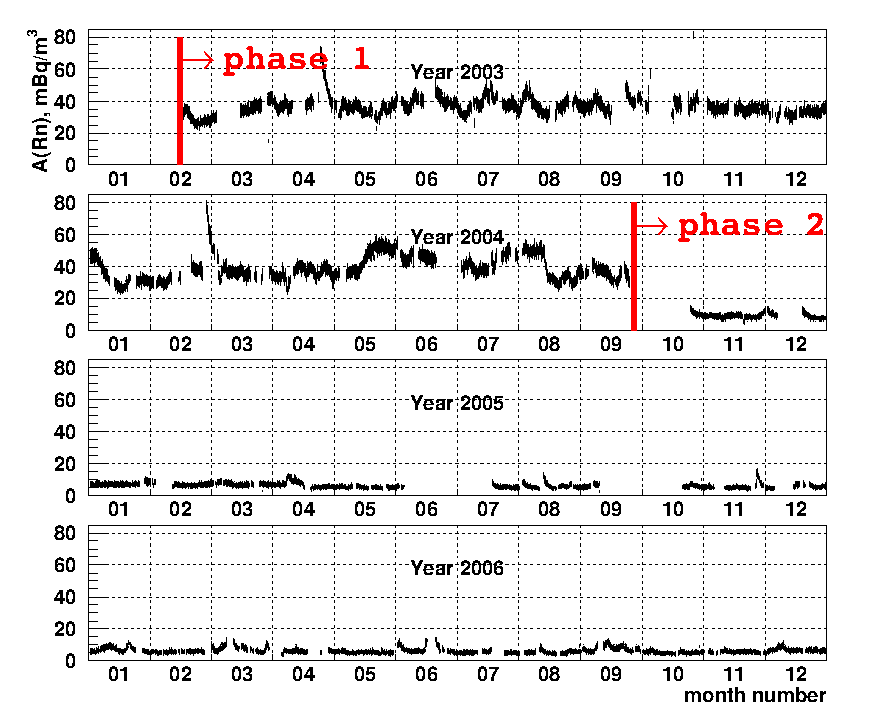
\includegraphics[scale=0.65]{pictures/Chap3/rn_bytime.pdf}
\caption{Radon activity measured in the NEMO-3 detector. The level of radon is reduced by a factor $\sim$~6. The time periods preceding and following the anti-radon facility are respectively referenced as Phase 1 and Phase 2.}
\label{RadonByTime}
\end{center}
\end{figure}


\FloatBarrier



\subsection{Results and measurements}


\NI After seven years of data taking, NEMO-3 has been stopped and disassembled. The strongest limit produced for 0$\nu\beta\beta$ comes from $^{\text{100}}$Mo, with a measurement of T$_{\text{1/2}}^{\text{0}\nu}$~>~1.1~$\times$~10$^{\text{24}}$~y corresponding to $\langle$m$_{\beta\beta}\rangle$~<~0.3~-~0.8~eV \cite{NEMO3:Mo100}.


\bigskip


\NI  The results on the searches for 2$\nu\beta\beta$ and 0$\nu\beta\beta$ are gathered in Table~\ref{tab:SummaryDecayRateNEMO3}. Most of these decays have been measured for the first time by NEMO-3 and some of them constitute the world's best measurements or limits. The last column of Table~\ref{tab:SummaryDecayRateNEMO3} presents the limit set on m$_{\beta\beta}$ in case of the 0$\nu\beta\beta$ is induced by the exchange of a light Majorana neutrino. These results have also been interpreted in the context of other models and limits have been set on different mechanisms such as the exchange of R-parity violating supersymmetric particles, right-handed currents and majoron emission \cite{Arnold2016bed,NEMO3:Nd150,NEMO3:Ca48,NEMO3:Mo100}. 


\bigskip


\begin{table}[h!]
\centering
%\begin{turn}{90}
\begin{tabular}{c|c|c|c|c|c}

Isotopes & Exp. [y] & T$_{\text{1/2}}^{\text{2}\nu}$ [y] 90 \% C.L. & T$_{\text{1/2}}^{\text{0}\nu}$ [y] 90 \% C.L. & m$_{\beta\beta}$ [eV] & ref\\

\toprule

$^{\text{100}}$Mo  & 4.96 & [7.1 $\pm$ 0.5] $\times$ 10$^{\text{18}}$ & > 1.1 $\times$ 10$^{\text{24}}$ & < [0.33 - 0.62] & \cite{NEMO3:Mo100} \\[0.1cm]

$^{\text{82}}$Se  & 5.25 & [10.07 $\pm$ 0.14 $\pm$ 0.54] $\times$ 10$^{\text{19}}$ & > 2.5 $\times$ 10$^{\text{23}}$  & < [1.2 - 3.0] &\cite{NEMO3:Se82}  \\[0.1cm]

$^{\text{130}}$Te & 3.49 &[7.0 $\pm$ 0.9 $\pm$ 1.1] $\times$ 10$^{\text{20}}$ & > 1.3 $\times$ 10$^{\text{23}}$  & - & \cite{NEMO3:Te130}\\[0.1cm]

$^{\text{116}}$Cd & 5.26 &[2.74 $\pm$ 0.04 $\pm$ 0.18] $\times$ 10$^{\text{19}}$ & > 1.0 $\times$ 10$^{\text{23}}$  & < [1.4 - 2.5] &\cite{Arnold2016bed} \\[0.1cm]

$^{\text{150}}$Nd & 5.25 &[9.34 $\pm$ 0.22 $\pm$ $^{+\text{0.62}}_{-\text{0.60}}$] $\times$ 10$^{\text{18}}$ & > 2.0 $\times$ 10$^{\text{22}}$  & [1.6 - 5.3] & \cite{NEMO3:Nd150}\\[0.1cm]

$^{\text{96}}$Zr  & 3.35 & [2.35 $\pm$ 0.14 $\pm$ 0.16] $\times$ 10$^{\text{19}}$ & > 9.2 $\times$ 10$^{\text{21}}$  & - & \cite{NEMO3:Zr96}\\[0.1cm]

$^{\text{48}}$Ca  & 5.25 &[6.4 $\times$ $^{+\text{0.7}}_{-\text{0.6}}$ $^{+\text{1.2}}_{-\text{0.9}}$] $\times$ 10$^{\text{19}}$ & > 2.0 $\times$ 10$^{\text{22}}$  & < [6.0 - 26] & \cite{NEMO3:Ca48}\\[0.1cm]

\bottomrule
\end{tabular}
%\end{turn}
\caption{Summary of the different half-lives measured for isotopes introduced in NEMO-3.}
\label{tab:SummaryDecayRateNEMO3}
\end{table}


\NI Thanks to the ability of NEMO-3 to fully reconstruct the events topology, more exotic searches can also be performed. Studies of the decays via the excited states and search for quadruple beta decay decay (0$\nu$4$\beta$) are ongoing~\cite{QuadrupleBetaDecayNEMO}. Chapter~6 presents the analysis done concerning the search for the $\beta\beta$ decays of $^{\text{116}}$Cd via the excited states of $^{\text{116}}$Sn.


\FloatBarrier


\section{The SuperNEMO demonstrator module}\label{sec:SuperNEMO}


\NI Based on the success of NEMO-3, a new detector with higher sensitivity, SuperNEMO, has been proposed. The goal of the SuperNEMO experiment is the search for the 0$\nu\beta\beta$ decays with a sensitivity of 10$^{\text{26}}$~y corresponding to m$_{\beta\beta}$ < 0.04 - 0.1~eV. The construction of a first SuperNEMO module called demonstrator is ongoing at LSM. It consists of a central frame supporting thin $\beta\beta$ foils surrounded by two trackers enclosed by a calorimeter as shown in Figure~\ref{SuperNEMOexplodedView}. The module is 4~m high, 6~m long and 2~m wide.


\bigskip


\NI An extended R\&D program has been performed in order to improve the detector design and its radiopurity to increase detector performance. This module will be used to validate all the design upgrades and verify that a very low level of background is achievable (10$^{\text{-4}}$~events/keV/kg/y in the region of interest) with such a large mass of detector and source foils. It will contain 7~kg of $^{\text{82}}$Se to reach a half-life sensitivity of $\sim$~6~$\times$~10$^{\text{24}}$~years, after 2.5~years of data-taking, in best case scenario.



\begin{figure}[h!]
\begin{center}
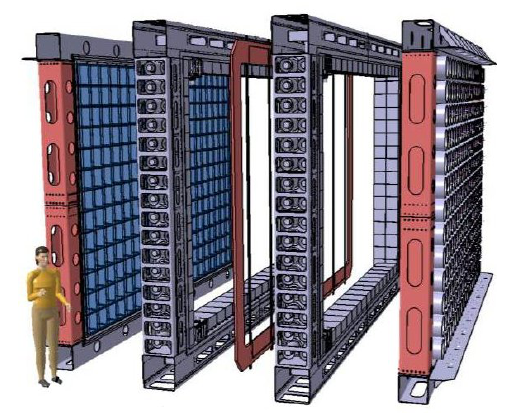
\includegraphics[scale=0.65]{pictures/Chap3/snemomodule.png}
\caption{Exploded view of one module of SuperNEMO. Thin source foils of $^{\text{82}}$Se are placed at the center of the detector. Two tracker modules made of 2034 Geiger cells reconstruct the electron tracks. Two calorimeter walls measure the energy of the electrons.}
\label{SuperNEMOexplodedView}
\end{center}
\end{figure}


\FloatBarrier


\subsection{Source foils}\label{sec:SourceFoilsSN}


\NI The demonstrator module will contain 7~kg of enriched $^{\text{82}}$Se. The choice of this isotope has been mainly motivated because none of its characteristics, phase space, NME, 2$\nu\beta\beta$ half-life and isotropic abundance, is an obstacle to the search for 0$\nu\beta\beta$. Futhermore its high end-point is far away from most of the background coming from radioactivity. To reach a sensitivity of $\sim$ 10$^{\text{26}}$~y in 500~kg~$\times$~y of exposure with $^{\text{82}}$Se the radio-purity level of the source foil in $^{\text{208}}$Tl and $^{\text{214}}$Bi must be better than 2~$\mu$Bq/kg and 10~$\mu$Bq/kg respectively~\cite{PhysicsCaseSuperNEMO}.


\bigskip


\NI The source is divided into 36 foils of~2.7~m long as shown in Figure~\ref{SuperNEMOFoils}. The 34 central foils are 13.55~cm wide, and the 2 border foils are 12.5~cm wide.


\begin{figure}[h!]
\begin{center}
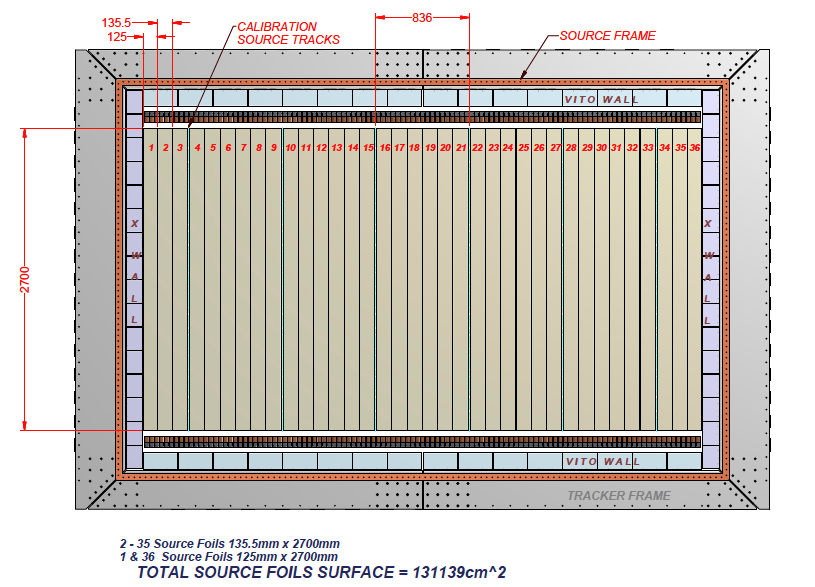
\includegraphics[scale=0.33]{pictures/Chap3/foil.png}
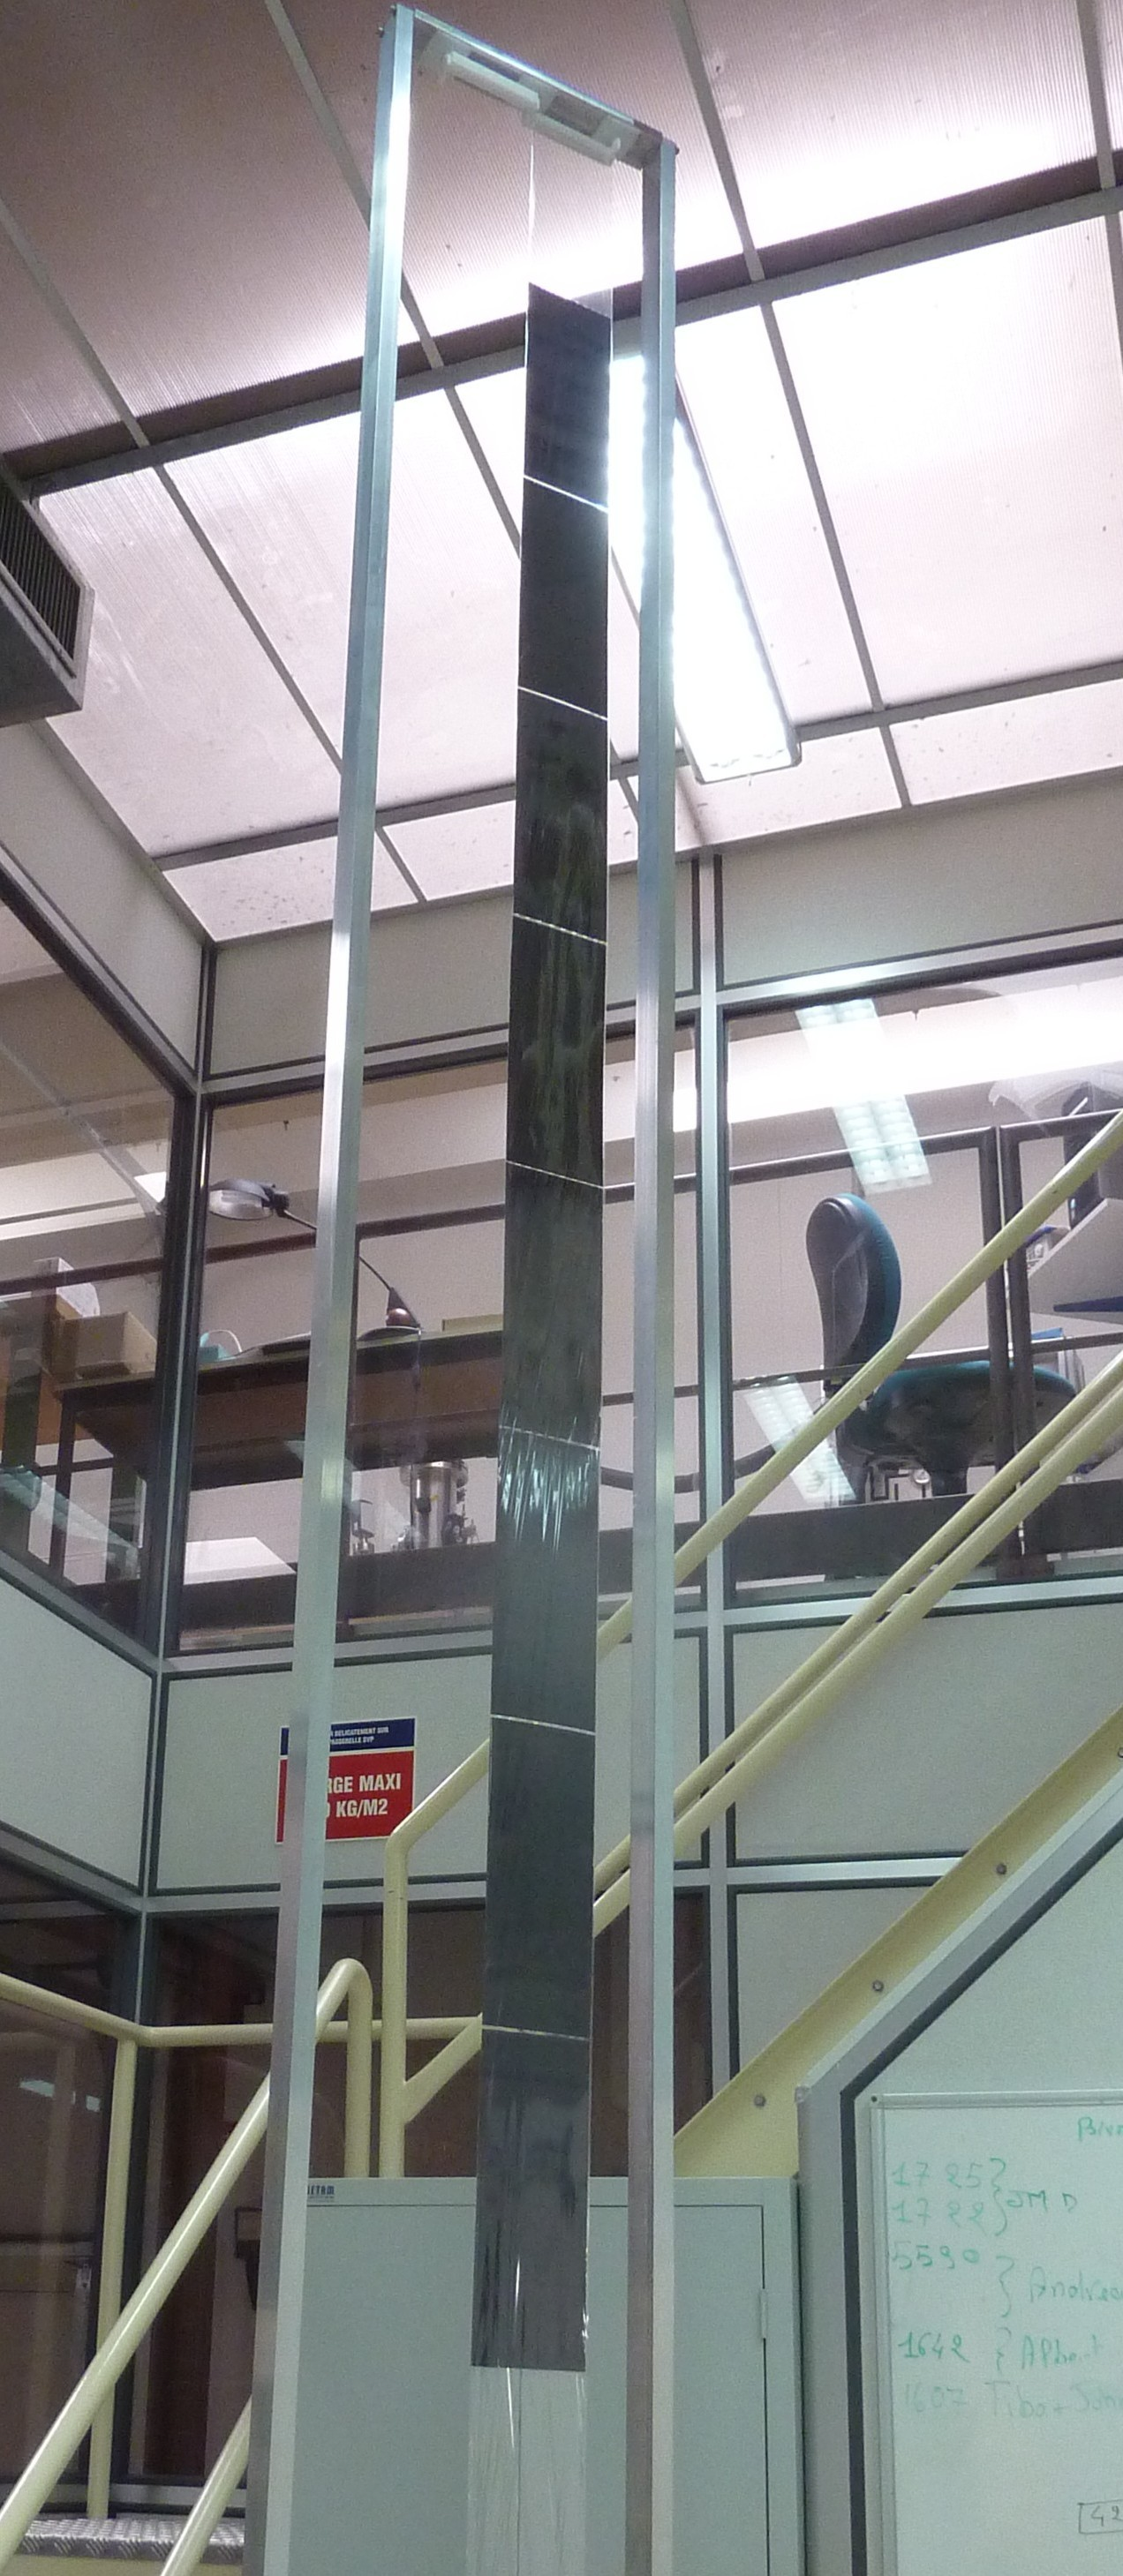
\includegraphics[scale=0.075]{pictures/Chap3/P1090162.JPG}
\caption{Left : Source plane design. It is divided in 36 foils
(34 with 13.55 cm width and 2 with 12.5 cm width). Right : Picture of one strip.} 
\label{SuperNEMOFoils}
\end{center}
\end{figure}


\NI They are composite foils with a surface densities of 40~-~60~mg/cm$^\text{2}$. The selenium is under a powder form which is mixed with a radiopure glue (PolyVinyl Alcohol~:~PVA) and ultrapure water to obtain a liquid paste. This paste is then spread out between two backing films made of 12~$\mu$m thick mylar sheets. However, the fabrication technique applied for NEMO-3 used perforated mylar backing film (section~\ref{sec:CdSectorInNEMO3}). The process to produces these holes can contaminate the source foil. It is in this optic that a new foil fabrication procedure has been proposed and studied. The new method consists of unmoulding the selenium foil and cut it into pads. These pads are then inserted into two raw mylar foils without micro-holes, joined with a weld as shown in Figure~\ref{SuperNEMOFoils}. Chapter~4 presents the work done concerning the design optimisation of the SuperNEMO source foil.

\bigskip


\NI To measure the very low purity of the foils (2$\mu$Bs/kg and 10$\mu$Bs/kg in $^{\text{208}}$Tl and $^{\text{214}}$Bi respectively), the NEMO collaboration decided to develop and build a dedicated detector called BiPo~\cite{BiPoDetector}. The concept of the BiPo detector is the identification of the so-called Bi-Po events which corresponds to the detection of an electron followed by a delayed $\alpha$ particle. For example, as shown in Figure~\ref{BiPoDecayChain}, in uranium decay chain, $^{\text{214}}$Bi is a $\beta$ emitter decaying to $^{\text{214}}$Po, which is itself an $\alpha$ emitter with a characteristic half-life of 164~$\mu$s. The BiPo technique consists in installing the material of interest between two thin ultra pure plastic scintillators. The $^{\text{208}}$Tl and $^{\text{214}}$Bi contaminations are measured by detecting the $\beta$-decay as an energy deposition in one scintillator and no coincidence signal from the opposite side, and the delayed $\alpha$ particle as a delayed signal in the second opposite scintillator without a coincidence in the first one. 


\begin{figure}[h!]
\begin{center}
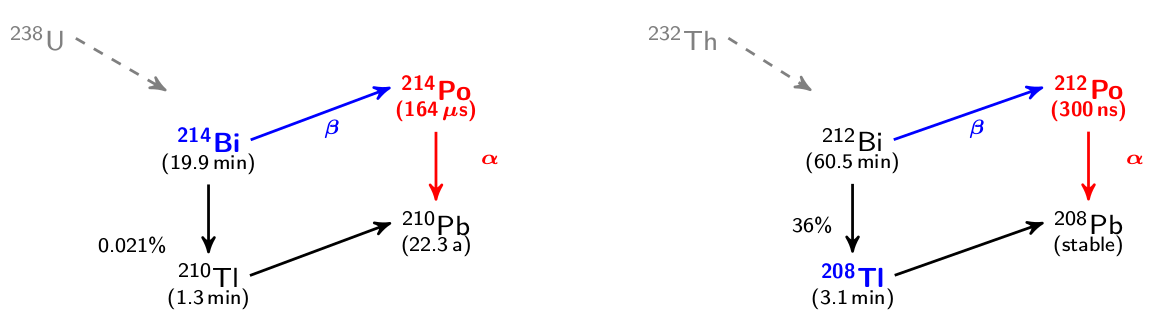
\includegraphics[scale=0.33]{pictures/Chap3/BiPoDecayChain.png}
\caption{The $^{\text{214}}$Bi$^{\text{214}}$Po and $^{\text{212}}$Bi$^{\text{212}}$Bi cascades used to measure the $^{\text{214}}$Bi and $^{\text{208}}$Tl contaminations.}
\label{BiPoDecayChain}
\end{center}
\end{figure}


\bigskip


\NI The BiPo detector has been installed in 2012 at Canfranc Underground Laboratory in Spain. It is made of 2 identical modules, each of them containing 40 scintillator blocks (coupled with 5'' PMTs). Each optical module covers an area of 30 $\times$ 30 cm$^\text{2}$, as presented in Figure~\ref{BiPoDetector}. This segmentation allows detection of possible hot spots on the foil. In a first step, the detector took data without any foils to measure its own level of background. The results of 0.16~$\mu$Bq/m$^\text{2}$ in $^{\text{214}}$Bi and 1.28~$\mu$Bq/m$^\text{2}$ in $^{\text{208}}$Tl allow to reach the expected sensitivity of 10 and 2~$\mu$Bq/kg in $^{\text{214}}$Bi and $^{\text{208}}$Tl, after a few months of data taking~\cite{BiPoDetector}. BiPo detector also measured different source foil components like the PVA or the Mylar film. The results of these measurements will be given in Chapter~4. F%inally, some final foils have been measured before introduction into in the demonstrator in order to validate their radiopurity. More details are given in Appendix~1.  


\begin{figure}[h!]
\begin{center}
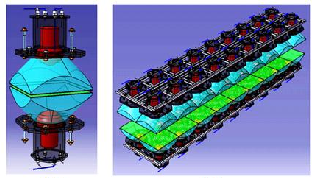
\includegraphics[scale=1.1]{pictures/Chap3/snemo_bipo.png}
\caption{Left : Pair of sub-modules coupled face to face. The green part represents the thin scintillators. The optical guides appear in blue and the PMTs in red. Right : assembly of the 40 optical sub-modules.}
\label{BiPoDetector}
\end{center}
\end{figure}



\FloatBarrier


\subsection{Tracker}


\NI The SuperNEMO tracker is similar in conception to the one of NEMO-3. It contains 2034~Geiger cells arranged in 9~layers parallel to the foil within a gas mixture of He~(95~\%), ethyl alcohol~(4~\%), Ar~(1~\%)~\cite{trackerSN}. Each cell is made of a 40~$\mu$m stainless steel central anode surrounded by eight 50~$\mu$m ground wires. To maintain the tracking properties of the detector, the mixture ratio of the gas must be kept constant. A gas system has been developed to ensure its mixture, purification, and flowing into the detector. The SuperNEMO tracker consists of an assembly of four parts called C-sections due to their C-shape. 


\bigskip


%An additional step forward in tracker production has been the design and construction
%of a wiring robot, which has automated the manufacturing process. This greatly
%reduces the risk of contamination of the 260,000 wires


\NI In order to reduce the risk of contamination of the wires, a wiring robot has been designed and built to automate the manufacturing process. A great care has also been taken concerning the radiopurity of the materials (copper, steel, duracon). Each of them has been tested in germanium detector. The construction of the basic units called cassettes and their assembly in the C frame took place under clean room conditions. To validate both the mechanical processes and the choice of the materials, radon emanation measurements of three of the four C-sections have been realized. The last C-section has not been measured condidering no changes in its material and production process. The results of these measurements are summarized in Table~\ref{tab:RadonEmanation}. Extrapolated to full demonstrator, a value of the activity of 0.21~mBq/m$^{\text{3}}$ can be obtained at nominal flowrate. The value of 0.12~mBq/m$^{\text{3}}$ can be achieved when the flush rate is at 1m$^{\text{3}}$/hr.


\begin{table}[h!]
\centering
\begin{tabular}{c|c}
\toprule
C-section & Radon emanation \\
\hline	
C0 & 11.37 $\pm$ 1.44~mBq \\
C1 & 15.26 $^{+\text{2.5}}_{\text{4.0}}$~mBq \\
C2 & 3.28 $\pm$ 1.39~mBq \\
\bottomrule
\end{tabular}
\caption{Summary of the radon emanation measurements of the different C-sections. The C3 has not been measured.}
\label{tab:RadonEmanation}
\end{table}


\bigskip


\NI The commissioning of the first C-section has been realized using cosmic muon events. Scintillator planes below the tracker volume were acting as a trigger. A picture of a C-section and cosmic muon event is shown in Figure~\ref{SnemoTracker}. Finally all the 2034 cells have been tested, 23~cells are considered as dead due to their triggering or a bad plasma propagation. The proportion of fully operational or recoverable channels is 99~\% over the first three tracker sections. 


\begin{figure}[h!]
\begin{center}
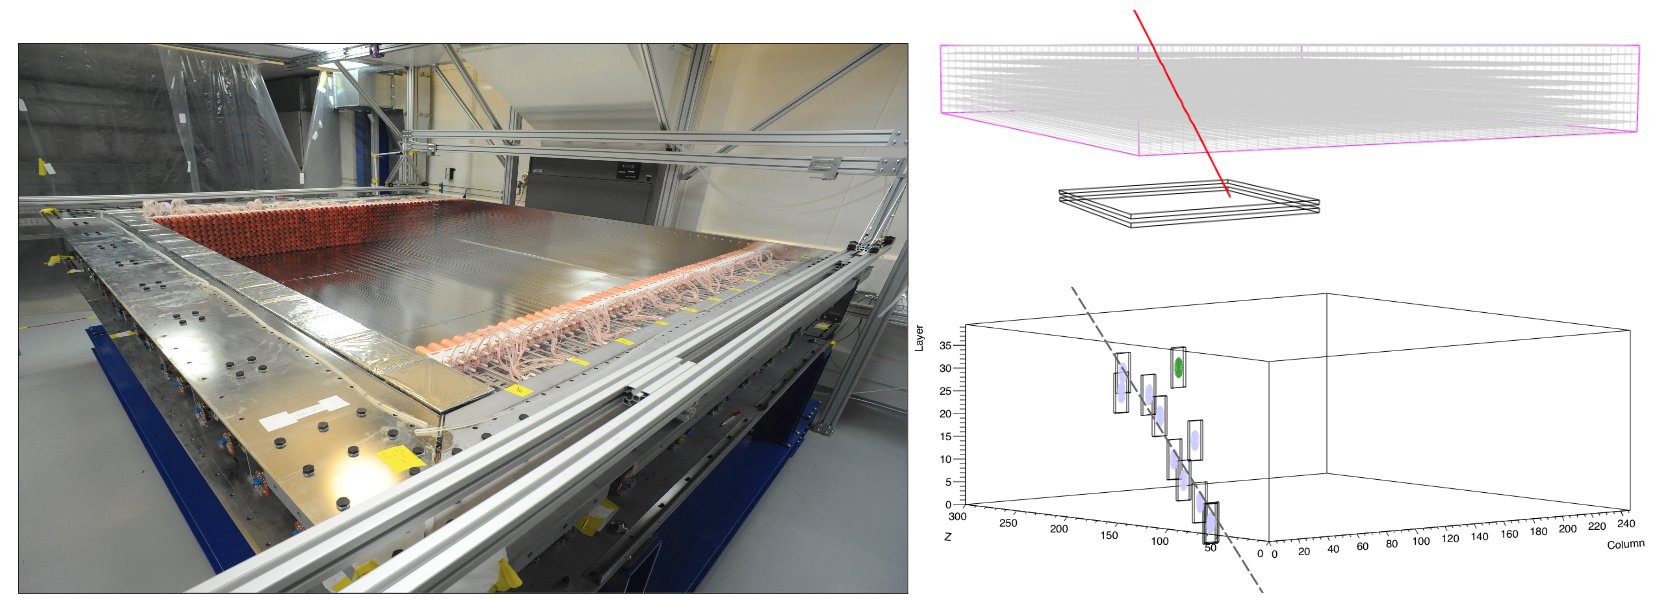
\includegraphics[scale=0.25]{pictures/Chap3/TrackerTestCosmic.png}
\caption{Left : picture of one of the four C-sections fully assembled. It is set horizontally, later in the SuperNEMO demonstrator, the Geiger cells will be vertical, parallel to the source foil. The copper parts are the end-caps supporting the wires. Top right : simulation of a cosmic muon crossing through the tracker. Bottom right : real cosmic muon event crossing the tracker.}
\label{SnemoTracker}
\end{center}
\end{figure}


\NI In order to improve the impermeability of the seals closing the tracking volume, especially to avoid radon diffusion coming from PMTs, the wire chamber will be isolated from the rest of the detector with a nylon radon-tight film. Futhermore, the entire detector will be inside a radon clean tent.


\FloatBarrier


\subsection{Calorimeter}


\NI The goals of the SuperNEMO calorimeter are the same than the NEMO-3 calorimeter, measure the energy and arrival time of particles and provide a fast trigger. The calorimeter of the SuperNEMO demonstrator is composed of 712 optical modules distributed in six walls~\cite{SNCalorimeter}.


\bigskip


\NI The two main walls are located on opposite sides of the source foil faces. Each main wall contains 260~polystyrene cubic scintillator blocks of 256~mm $\times$ 256~mm $\times$ 194~mm, coupled to 8'' low radioactive PMT (R5912-03). The main difference with the NEMO-3 blocks is that the PMT is directly coupled to the scintillator block as shown in Figure~\ref{SnemoOpticalModule}. Futhermore, the polystyrene scintillators used in NEMO-3 have been replaced with poly-vinyl toluene (PVT). Thanks to this new design the energy resolution has been improved by a factor two, the FWHM has been measured to be 8~\% at 1~MeV~as shown in Figure~\ref{EnergyResolutionCaloBlock}~\cite{SNCalorimeter}.



\begin{figure}[h!]
\begin{center}
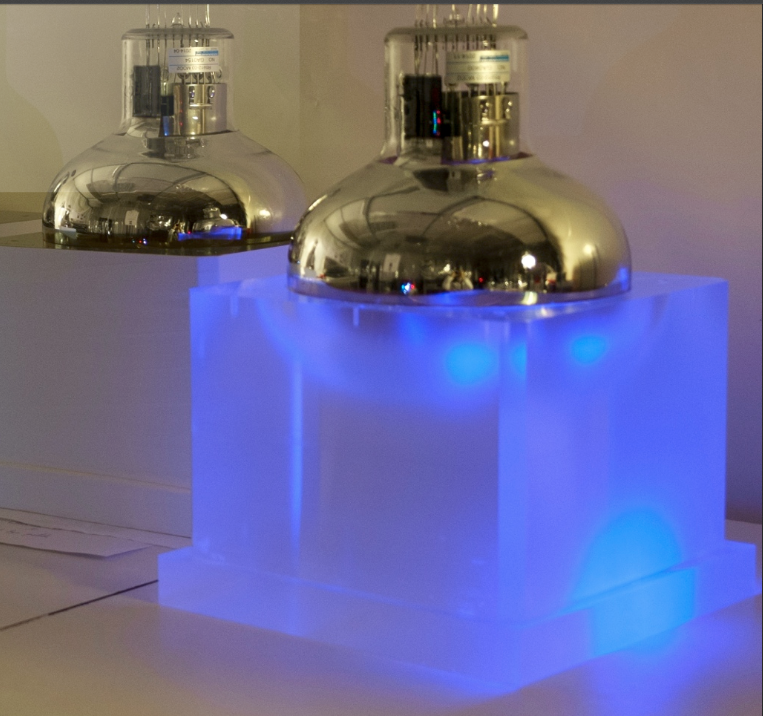
\includegraphics[scale=0.25]{pictures/Chap3/calo_1.png}
\caption{Optical module composing the calorimeter before being wrapped into teflon and mylar. The scintillator block is directly coupled to the PMT.}
\label{SnemoOpticalModule}
\end{center}
\end{figure}


\begin{figure}[h!]
\begin{center}
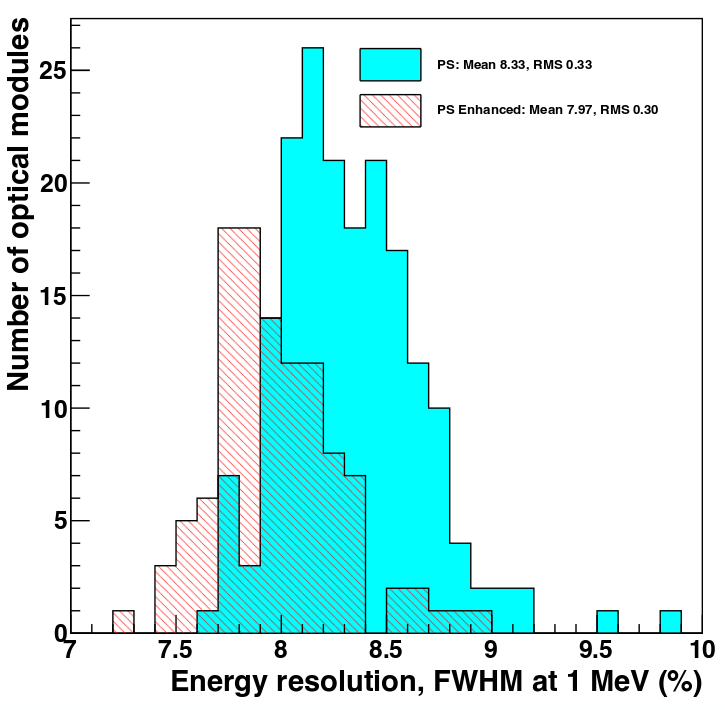
\includegraphics[scale=0.25]{pictures/Chap3/EnergyResolution.png}
\caption{Energy resolution of the optical modules.}
\label{EnergyResolutionCaloBlock}
\end{center}
\end{figure}



\NI The calorimeter is completed with two $\gamma$-veto capping the top and the bottom of the detector containing 64~plastic scintillator blocks of 210~mm $\times$ 200~mm $\times$ 145~mm. These blocks are coupled to 5'' PMTs (R6594). Finally, two x-walls cover the sides of the detector. They are made of 32~plastic scintillator blocks (290~mm $\times$ 304~mm $\times$ 145~mm) also coupled to 5'' PMT. Note that the first and last rows of the main wall are coupled with 5''~PMTs since these blocks are partially covered by the $\gamma$-veto and will probably not be used for the analysis.

\bigskip


\NI To improve the light collection, all the block sides are wrapped into teflon film while the entry face is covered by 6~$\mu$m of aluminized mylar. Figure~\ref{SnemoCaloFrontView} is a picture of the SuperNEMO main wall during its construction at LSM. %A radon-free air will be introduced very close to the PMT to avoid high radon concentration coming from PMT emanations.


\begin{figure}[h!]
\begin{center}
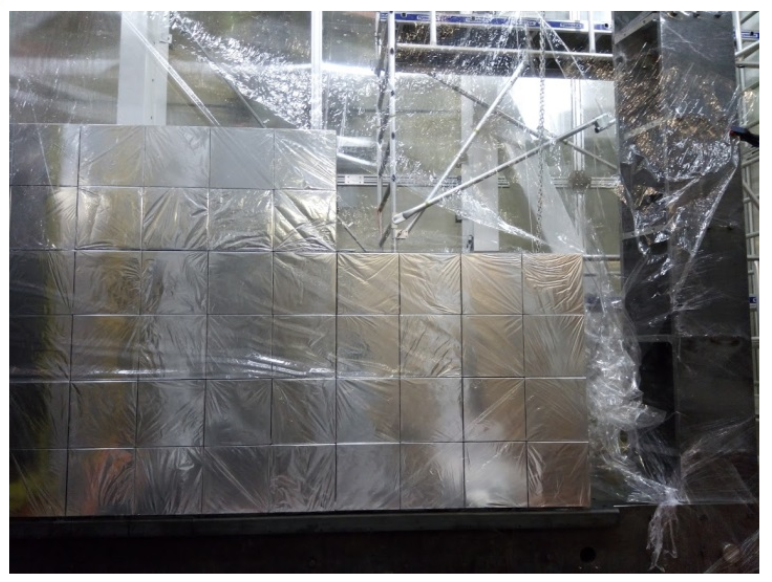
\includegraphics[scale=0.5]{pictures/Chap3/FrontViewCalo.png}
\caption{Front view of one main wall during its assembly at LSM. The wall is built by assembling the bricks (8 by 8).}
\label{SnemoCaloFrontView}
\end{center}
\end{figure}

\FloatBarrier


\subsection{Calibration system}


\NI The strategy to calibrate both energy and time is the same as that used in NEMO-3. Monthly, during dedicated runs, $^{\text{207}}$Bi sources will be introduced in the detector to calibrate the absolute energy scale. Between these runs, the response and the linearity will be monitored daily. 


\bigskip


\NI An improvement in the calibration system consists of the removal of the calibration tubes in which the sources were introduced. In this new automated system, the $^{\text{207}}$Bi sources are guided into position thanks to a system of weights and stepper motors. In this way, no material will remain in the detector outside the calibration runs.


\bigskip


\NI To monitor the response of the optical modules a light injection system has been developed. The idea is exactly the same as it was with the NEMO-3 laser survey using LEDs instead of lasers. A schematic view of the light injection system is presented in Figure~\ref{LIschema}. 20 UV LEDs will inject pulsed LED light into each scintillator blocks via optical fibers. A reference optical module is used to monitor the light level against a $^{\text{241}}$Am source.


\bigskip
\begin{figure}[h!]
\begin{center}
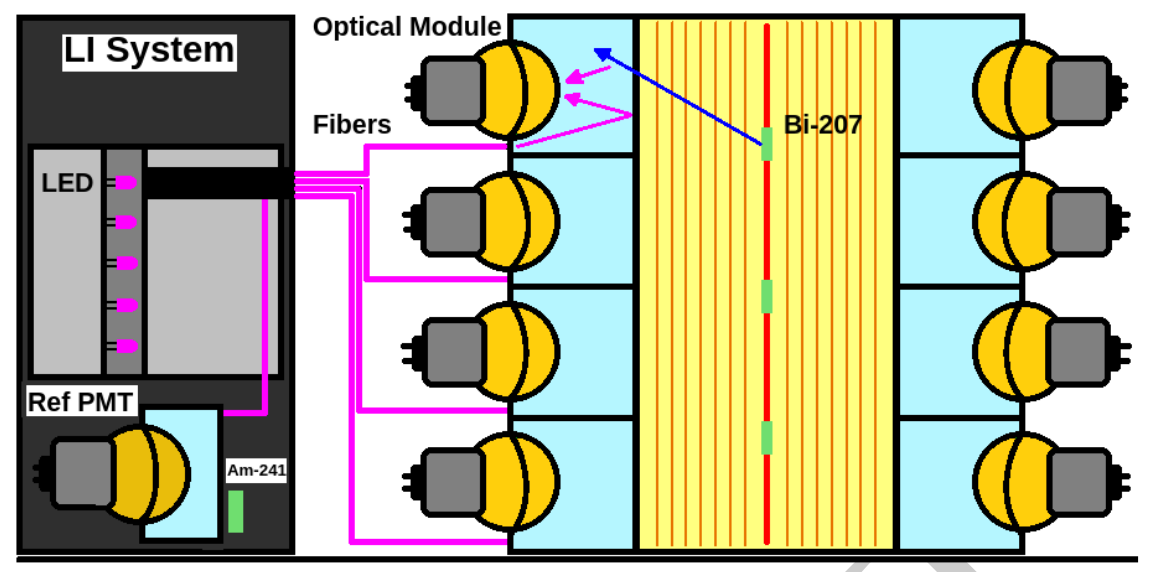
\includegraphics[scale=0.3]{pictures/Chap3/LIschema.png}
\caption{Schematic representation of the light injection system. Installed in an independant rack, a pulser will send into each optical module UV light via optical fibers. A reference PMT coupled to an americium-241 source is used to control the light level.}
\label{LIschema}
\end{center}
\end{figure}


\subsection{Shieldings}


\NI The strategy to protect the detector against the neutron and $\gamma$-ray fluxes is similar to the NEMO-3 strategy. Multilayer shields made of iron (20~cm), paraffin (20~cm), borated water (20~cm) and wood (30~cm) will surround the detector to reduce photon and neutron fluxes coming from the rocks of the laboratory. Finally, to minimise radon diffusion an anti-radon tent will surround the detector and will be constantly flushed with filtered air.


\subsection{Prospectives}


\NI The construction of the demonstrator began with most of the different components already manufactured and present at LSM. The first and second calorimeter walls were built between the end of 2016 and the beginning of 2017. Two C-sections have been assembled and coupled to the first calorimeter wall to form a half-detector. The installation of the source foils is planned by autumn of 2017.% , just after the source deployment system. The gas system has been installed.

\bigskip


\NI In case the demonstrator module is successful, other SuperNEMO like modules could be deployed. The goal would be to investigate 0$\nu\beta\beta$ with 100~kg of $^{\text{82}}$Se to reach a half-life sensitivity of~10$^{\text{26}}$~years, corresponding to an effective neutrino mass of 50~-~100~meV. The 100~kg of $^{\text{82}}$Se could be divided between 20 identical and independent modules, in a way to provide flexibility in the modules location as they can be arranged to maximise the available space in underground laboratories. As the source is decoupled from the detector, other isotopes as $^{\text{150}}$Nd and $^{\text{48}}$Ca could also be introduced.


\bigskip


\NI Table~\ref{tab:DifferenceNEMO3-SuperNEMO} summaries key experimental achievements of NEMO-3 and the target levels for SuperNEMO to reach the sensitivity of~10$^{\text{26}}$~years. 


\begin{table}[h!]
\centering
\begin{tabular}{c|c|c}
\toprule
      & NEMO-3 & SuperNEMO \\
\hline
Mass~[kg] (main isotopes)           & 7 ($^{\text{100}}$Mo)         & 100 ($^{\text{82}}$Se)        \\[0.1cm]
 T$_{\text{1/2}}^{\text{2}\nu}$ [y] & 7.2 $\times$ 10$^{\text{18}}$ & 9.9 $\times$ 10$^{\text{19}}$ \\[0.1cm]
\hline
Energy resolution & & \\
FWHM at 1~MeV                       & 15~\%                         & 8~\%                          \\[0.1cm]
FWHM at 3~MeV                       & 8~\%                          & 4~\%                          \\[0.1cm]
\hline
Source radiopurity & & \\
A($^{\text{208}}$Tl)               & $\sim$ 100 $\mu$Bq/kg         & $<$ 2 $\mu$Bq/kg               \\[0.1cm]
A($^{\text{214}}$Bi)               & < 300 $\mu$Bq/kg              & < 10 $\mu$Bq/kg                \\[0.1cm]
\hline
Level of radon A($^{\text{222}}$Rn)& $\sim$ 5.0 mBq/m$^\text{3}$ y   & < 0.1 mBq/m$^\text{3}$ y     \\[0.1cm]
\hline
Sensitivity after 5~y of data taking & T$_{\text{1/2}}^{\text{0}\nu}$ > 10$^{\text{24}}$ & T$_{\text{1/2}}^{\text{0}\nu}$ > 10$^{\text{26}}$     \\[0.1cm]
\bottomrule
\end{tabular}
\caption{Summary of the key experimental achievements of NEMO-3 and the target levels for SuperNEMO.}
\label{tab:DifferenceNEMO3-SuperNEMO}
\end{table}  


\FloatBarrier


\end{document}
